\documentclass[11pt]{My_preprint}

\title{
    Buoyancy driven motion of non-coalescing inertial drops: microstructure modeling with nearest particle statistics. 
}

\author[1,2]{Nicolas Fintzi}
\author[1]{Jean-Lou Pierson}
\author[2]{Stephane Popinet}
\affil[1]{IFP Energies Nouvelles, Rond-point de l’echangeur de Solaize, 69360 Solaize}
\affil[2]{Sorbonne Universit\'e, Institut Jean le Rond d'Alembert, 4 place Jussieu, 75252 PARIS CEDEX 05, France}
\normalmarginpar


\begin{document}

\maketitle

\begin{abstract}
    In this study, we analyze the various arrangements that droplets can form within dispersed buoyant emulsions, which we refer to as the study of microstructure. 
    To this end, we have developed a novel algorithm that effectively prevents numerical coalescence between drops while maintaining a reasonable computational cost. 
    This algorithm is integrated into the Volume of Fluid (VoF) method and implemented using the open-source code \href{http://basilisk.fr}{http://basilisk.fr}. 
    Subsequently, we perform Direct Numerical Simulations (DNS) of statistically steady state mono-disperse buoyant emulsion over a broad range of dimensionless parameters, including the particle volume fraction ($\phi$), the Galileo number ($Ga$) and the viscosity ratio ($\lambda$). 
    We make use of nearest particle statistics to quantify the microstructure properties.  
    As predicted by \citet{zhang2023evolution}, it is demonstrated that the second moment of the nearest particle pair distribution can effectively quantify microstructural features such as particle clusters and layers. 
    Specifically, the findings are: (1) In moderately inertial flows ($Ga=10$), droplets form isotropic clusters. 
    In high inertial regimes ($Ga=100$), non-isotropic clusters, such as horizontal layers, are more likely to form. 
    (3) The viscosity ratio plays a significant role in determining the microstructure, with droplets that are less viscous or equally viscous as the surrounding fluid tending to form layers preferentially. 
    Overall, our study provides a quantitative measure of the microstructure 
     in terms of $Ga$, $\phi$ and $\lambda$. 
\end{abstract}

\section{Introduction}
\section{Introduction}



\begin{enumerate}
    \item[Intro : ]
    Buoyancy-driven droplet flows are encountered in many chemical engineering processes such as gravity separators, liquid-liquid extractors, etc. The usual engineering practice to model such facilities is to make use of the averaged Navier-Stokes equations and population balance equations. 
    \item[Why is it interesting :]
    However, these methods necessitate closure laws and a deep understanding of particle pair statistics.
    Especially, closures laws are in fact microstructure dependent. 
    Therefore, in an objective to understand to physics these terms it is primordial to understand the microstructure and why it is like so. 
    \item[bibliography : ]
    Previous authors investigated the microstructure of bubbly flows. 
    \citet{bunner2002dynamics} reported the creation of horizontal raft for rising  spherical bubbles. 
    \citet{bunner2003effect} demonstrated taht due to wake trapping effect deformable bubbles have a tendency to align horizontally. 
    In a more recent study \citet{zhang2021direct} also found the creation of horizontal layers of particles. 
    Regarding the solid particles other studies have been conducted for the sedimentation of spheres \citet{shajahan2023inertial}, and they found a high probability of particle pair on  the side of the particle of reference.     
    \item[What is still needed :]
    None, of these studies focus on droplets' suspension. 
    So no closure are available. 
    Additionally, none of them proposed an algorithm to avoid coalesce. 
    \item[What good if i new :]
    An algorithm to prevent coalesce would allow us to perform DNS for arbitrary long time with a fixed population of droplets. 
    In addition to providing data for the closure terms appearing in averaged models, the simulations are of great interest to understand and describe the microstructure of suspensions. 
    \item[introduce the plan :]
    Therefore, within a multiscale strategy, we perform tri-periodic Direct Numerical Simulations (DNS) of monodisperse buoyancy driven suspension of drops.
    In this work we present a concise analysis of the microstructure by analyzing the \textit{Nearest Particle Statistics} recently revisited by \citet{zhang2021ensemble}. 
    We start in \ref{sec:methodo} to present the DNS methodology. 
    Then, we introduce quickly the \textit{nearest particle statistics}.
    In \ref{sec:microstructure} we present an analysis of the microstructure geometry and identify structure such as layers and cluster with respect to the dimensionless parameters. 
    Then, in \ref{sec:time} we describe the relevant timescale of the flow. 

\end{enumerate}

\section{Numerical methodology}
\label{sec:methodo}

This section outlines the approach employed for performing simulations to achieve statistically steady states in the context of a rising mono-disperse suspension of droplets within a fully periodic domain.
We start by presenting the relevant physical parameters, followed by an overview of the numerical methods employed.
Finally, we detail the methodology implemented for collecting statistical data on microstructure, which will be presented in the following sections.

%In this section we expose the strategy employed to conduct statistically steady state simulations of rising mono-disperse suspension of droplets in a fully periodic domain. 
%We start by introducing the physical parameter, followed by a description of the numerical methods.
%Lastly, we detail the methodology adopted to collect statistics about microstructure, which are presented in the next sections.

%The source code used to perform the DNS is entirely open source.
%The simulations are running within the \texttt{Basilisk C} framework, (see \href{http://basilisk.fr}{basilisk.fr}), which is an extension of the C programming language, adapted for the solution of partial differential equations on Cartesian meshes. 
%Note that this section is complemented by the wiki page, \href{http://basilisk.fr/sandbox/fintzin/Rising-Suspension/RS.c}{RS.c}, where the reader can access the source code used to conduct the DNS, as well as comments and notes to help comprehension. 

\subsection{Problem statement}

We investigate numerically the dynamics of homogeneous mono-disperse emulsions subject to buoyancy forces in a fully periodic domain. 
The dispersed and continuous phases are considered Newtonian fluids defined by viscosity $\mu_d$ (resp. $\mu_f$) and density $\rho_d$ (resp. $\mu_f$).
Throughout this work, the subscript $_d$ and $_f$ indicate properties belonging to the dispersed and continuous phases, respectively. 
The interface between both fluids is considered infinitely thin, free of impurities, and characterized by a constant surface tension $\gamma$. %with a coefficient  is assumed. 
The density and viscosity will be considered constant in each phase.
In dimensionless form, this problem is completely characterized by six dimensionless parameters:  the viscosity and density ratio, $\lambda = \mu_d / \mu_f$ and $\zeta = \rho_d / \rho_f$,  
the \textit{Galileo} number, 
\begin{equation*}
    Ga =\frac{\sqrt{\rho_f(\rho_f - \rho_d) g d^3}}{\mu_f},
\end{equation*}
the \textit{Bond} number, 
\begin{equation*}
    Bo =\frac{(\rho_f - \rho_d) g d^2}{\gamma},
\end{equation*}
the number of droplets per domain $N_b$, and the dispersed phase volume fraction $\phi$. 
Here, $d$ represents the diameter of a sphere with the same volume as the droplets and $g$ denotes the acceleration of gravity.
The \textit{Galileo} number measures the strength of the buoyancy forces relative to the viscous forces, whereas the \textit{Bond} number evaluates the ratio between buoyancy and capillary forces. 

%To provide a brief overview of the range of interest for these numbers in an industrial context, let us consider the example of a vegetable oil/water system.
%In most liquid-liquid system encountered in industrial processes the diameter of the droplets lies in the range $d = [50 \mu \text{m}, 3 \text{mm}]$. To provide order of magnitude of the quantities of interest let us consider the example of a vegetable oil dispersed in water. The density and viscosity of the continuous phase are approximately $\rho_f = 1000 \text{kg/m}^3$ and $\mu_f = 10^{-3} \text{Pa.s}$, respectively. The density and viscosity of the dispersed phase are close to $\rho_d = 900 \text{kg/m}^3$ and $\mu_d = 10^{-2} \text{Pa.s}$, respectively.
%We consider the gravitational acceleration on earth, thus $g= 9.81 \text{m.s}^{-2}$.
In most liquid-liquid systems encountered in industrial processes, the droplet diameters typically range from 10 micrometers to a few millimeters. To illustrate the order of magnitude of the relevant quantities, consider a scenario where vegetable oil is dispersed in water. The continuous phase (water) has a density of approximately $\rho_f = 1000 \text{kg/m}^3$ and a viscosity of about $\mu_f = 10^{-3} \text{Pa.s}$. In contrast, the dispersed phase (vegetable oil) has a density close to $\rho_d = 900 \text{kg/m}^3$ and a viscosity around $\mu_d = 10^{-2} \text{Pa.s}$.
The surface tension of the oil/water system is approximately $\gamma = 0.05 \text{N.m}^{-1}$. The maximum allowable volume fraction is set at $\phi = 0.2$. Beyond this value, particles tend to coalesce easily, leading to a loss of the dispersed flow topology.%The maximum volume fraction is set to $\phi = 0.2$, indeed above such $\phi$ particles coalesce easily and the topology of the flow cannot be considered as dispersed anymore. %\citep{de2015gouttes}. 
\begin{table}[h!]
    \centering
    \caption{Dimensionless parameters of a water/oil system.}
    \begin{tabular}{|c||c|c|c|c|c|}
        \hline&$Ga$&$Bo$&$\phi$&$\lambda$&$\zeta$\\ \hline
        \hline Oil/Water&$[0.35,160]$&$[10^{-5};10^{-1}]$&$<0.2$&$10$&$0.9$\\ \hline
    \end{tabular}
    \label{tab:parameters_exp}
\end{table}
\ref{tab:parameters_exp} gives the corresponding dimensionless parameters.  
Notice that the \textit{Bond number} is relatively low, indicating that the droplets are nearly spherical in these processes.
Following \ref{tab:parameters_exp}, to approach real-life applications, we conducted DNS for four volume fractions, specifically $\phi = 0.01,0.05,0.1,0.2$.
In contrast to most previous studies, we keep the number of droplets constant while changing the volume fraction $\phi$. 
We then modify the domain size $\mathcal{L}$ accordingly. 
This introduces another dimensionless parameter of interest: $\mathcal{L}/d$, which measures the confinement of the particles within the finite numerical domain. 
This parameter is purely determined by $\phi$ and $N_b$, and will thus be refereed as a \textit{secondary parameter}.

As mentioned, the \textit{Bond} numbers of our targeted application is very low.
Therefore, the \textit{Bond} number is set to $Bo = 0.2$, and it will stay constant throughout this study.
DNS with lower \textit{Bond} numbers become excessively expensive due to the restrictive capillary time step constraint. 
However, we assert that for $Bo \leq 0.2$, the droplet shape essentially remains spherical, at least for small \textit{Galileo} numbers. 
Additionally, the ratio between inertia and surface tension forces is given by the \textit{Weber} number, 
\begin{equation*}
    We = \frac{\rho U^2d}{\gamma}%\frac{Bo \cdot Re^2}{Ga},
\end{equation*}
%where $Re = \frac{\rho_f d U}{\mu_f}$ is the Reynolds number based on 
where $U$ is the relative velocity which is the difference between the dispersed phase velocity and the continuous velocity.%drift velocity $U$ which is the difference between the dispersed phase velocity and the bulk velocity.
%Values of \textit{Reynolds} numbers for each DNS are provided in \ref{ap:slip_vel} (\ref{fig:Reall}). 
Extreme values of $We$ reached in these simulations are displayed in \ref{tab:simulations}. 
It is clear that for $We=0.6$, we might expect some deformations; nevertheless, in most cases, $We$ stays below these values. 
Consequently, whether in the viscous or inertial regimes, the droplets are expected to remain spherical according to the values of $Bo$ and $We$.
This statement is verified in appendix \ref{ap:deformation}.%will be verified in \ref{sec:microstructure}. 

%Density and viscosity ratio of droplets in real life applications are reported in \citet[Figure 1.]{balla2020effect}.
%As depicted in \citet[Figure 1.]{balla2020effect}, the viscosity and density ratio of fluid-fluid systems range between, $\lambda \in [10^{-4} : 10^4]$ and $\zeta \in [10^{-1} : 10^1]$, respectively. 

The study's primary objective is to investigate the microstructure through the nearest particle pair distribution function.
Thus, obtaining a sufficient number of DNS samples is crucial to ensure statistical convergence. 
Also, the physical quantities measured in the simulations must remain independent of the domain size. 
Therefore, we use a number of particles per domain of $N_b = 125$, roughly what \citet{hidman2023assessing} used for their DNS of fully-periodic buoyant rising bubbles.
Moreover, each DNS lasts for a time: $t^*_\text{end} = 1500 \sqrt{d/g}$.
% It is shown in \ref{ap:validation} that these parameters  are sufficient to obtain well converged statistics.  
\begin{table}[h!]
    \centering
    \caption{Dimensionless parameter range investigated in this work.}
    \begin{tabular}{|ccccccc|ccc|}\hline
        \multicolumn{7}{|c|}{Primary parameters}&\multicolumn{3}{|c|}{Secondary parameters}\\\hline\hline
        $Ga$&$Bo$&$\phi$&$\lambda$&$\zeta$&$N_b$&$t^*_\text{end}$&$\mathcal{L}/d$&$Re$&$We$\\ \hline
        $5\rightarrow 100$&$0.2$&$1\% \rightarrow 20\%$&$10$ \& $1$&$0.9$&$125$&$1500$&$6.7\to 18.7$&$10^{-1}\to 170$&$10^{-4}\to 0.6$\\ \hline
    \end{tabular}
    \label{tab:simulations}
\end{table}
This study presents DNS results with dimensionless parameters in ranges outlined in \ref{tab:simulations}.
In summary, we investigated $5$ \textit{Galileo} number $Ga = 5,10,25,50,100$, $4$ different volume fractions $\phi = 0.01,0.05,0.1,0.2$, and two viscosity ratios $\lambda =1,10$ with $Bo = 0.2$ and $\zeta = 0.9$. %In this study we restrict our attention to a single density ratio, $\zeta = 0.9$.
%Regarding the viscosity ratio, we accomplished DNS for 2 different values, namely $\lambda = 1,10$.
%Lastly, to explore the effect of inertia on the microstructure, the \textit{Galileo} number will vary within the range $Ga \in [5,100]$.
This makes a total of $40$ representative simulations of $N_b = 125$ droplets which last for $t= 1500 \sqrt{d/g}$. 
\subsection{Numerical method}

In this problem, the governing equations consist of the one-fluid formulation of the mass and momentum equation, with an additional transport equation for the dispersed phase indicator function. 
We recall their form here, 
\begin{align}
    \pddt \rho+ \div(\rho\textbf{u})
    &= 0,\\
    \label{eq:dt_urho}
    \pddt (\rho \textbf{u})
    + \div (\rho  \textbf{u} \textbf{u} - \bm\sigma)
    &= (\avg{\rho} - \rho)\textbf{g}
    + \textbf{f}_\gamma,\\
    \label{eq:dt_C}
    \pddt C + \textbf{u}\cdot\grad C  
    &= 0,
\end{align}
% \tb{mettre le link navier stokes solver et faire ca pour le reste }
which are the mass, momentum and colors function transport equation, respectively. 
The scalar fields $C$, represents the color function, which range between $0$ and $1$ to indicate the proportion of fluid and dispersed phase, respectively. 
We introduced the fluid velocity vector $\textbf{u}$ and the Newtonian stress tensor $\bm{\sigma} = -p \textbf{I} + \mu (\grad \textbf{u}+ \grad \textbf{u}^\dagger)$ where $p$ is the pressure fields and $^\dagger$ represents the transpose operator.
Note that the material properties, $\rho$ and $\mu$, take the value of the phases in presence, following the arithmetic average : $\rho = (1-C)\rho_f + C \rho_d$ and $\mu = (1-C)\mu_f + C \mu_d$. 
In our case the arithmetic mean turns out to perform better compared to the harmonic mean, which is often used to interpolate the viscosity for bubbly flows \citet{hidman2023assessing,innocenti2020direct}.
More details about this choice is provided in \ref{ap:validation} (\textit{Case 1.}). 
The capillary force is defined as, $\textbf{f}_\gamma =\textbf{n} \gamma \div \textbf{n} $, where \textbf{n} is the normal at the interface.
Following  \citep{bunner2002dynamics}, we incorporated the artificial body force term, $\avg{\rho}\textbf{g}$, on the right-hand side of \ref{eq:dt_urho}, to maintain a zero-averaged velocity throughout the entire numerical domain.  

To solve these equations we first initialized $125$ spherical droplets within a cubic domain with fully periodic boundary condition. 
We used the open source code \url{http///basilisk.fr} to discretize the governing equations in a multigrid solver. 
The Navier-Stokes equations are discretized with a centered scheme.
The two-phase flow solver uses the Volume of Fluid (VoF) method. 
The interfaces between the droplets and the carrier fluid is reconstructed using the Piecewise Linear Inter-face Calculation or PLIC method \citet[Chapter 5.]{tryggvason2011direct}.
Regarding the treatment of the surface tension force term we refer the reader to \citet{popinet2018numerical} for more details. 
The Basilisk solver has been validated extensively, in the framework of bubbly flow. 
Most of the previous studies \citep{hidman2023assessing,innocenti2020direct} recommend a grid definition of $\Delta/d \ge  30$, where $\Delta$ is the grid spacing. 
In \ref{ap:validation} we carried a mesh independence study and demonstrate that a grid spacing of $\Delta = d/30$ is also suitable in our context.
For readers seeking more detailed information about the solvers, we recommend the wiki pages : \href{http://basilisk.fr/src/navier-stokes/centered.h}{centered.h}, \href{http://basilisk.fr/src/tension.h}{tension.h} and \href{http://basilisk.fr/src/poissson.h}{poissson.h} where he can find the source code of the Navier-Stokes, surface tension and multigrid solver used in this work, respectively. 

With the VoF method droplets and bubbles may experience premature coalesce.
For a detailed discussion on this issue, see  \citet[Appendix B]{innocenti2020direct}.
However, in this work, it is imperative to conserve a specific (mono-disperse) population of droplets over time to accumulate sufficient statistics about the microstructure.
To tackle this issue we present in the next section a novel algorithm which prevent coalescence between droplets, while maintaining a reasonable cost. 






\subsection{The \texttt{no-coalescence.h} algorithm}

In previous studies various methods have been used to avoid coalescence. 
One method is to increase artificially the surface tension coefficient at the interface contact points, as demonstrated in the recent study of \citet{hidman2023assessing}.
% This method seems highly efficient, in terms of simplicity and computational expenses. 
However, it remains unclear if the physical behavior of the droplets interactions is well captured due to the introduction of artificial forces. 
Additionally, its applicability for denser emulsions, up to $\phi = 0.2$, remains uncertain. 
\citet{balcazar2015multiple} developed a multiple-marker level-set method to prevent coalescence, while \citet{zhang2021direct} used a multi-VoF method. 
The latter method consists in assigning to each droplet a different color function so  that the interfaces are reconstructed independently when droplets are in close contact.
Since the representations of the interfaces are independent, droplets in contact never coalesce.  
The latter method may be suitable for our objectives, however, it can be quite expensive as it requires solving a transport equation for each tracer, with one tracer assigned per droplet, meaning $125$ tracers in our case. 
\citet{karnakov2022computing} developed a multi-VoF method which requires a fixed number of tracers for an arbitrary number of droplets.
This approach allows multiple non-touching droplets to belong to the same field, which makes it more efficient than the previous study.
Although this approach shares the same basic principle with the one used here, i.e. coloring adjacent droplets with different colors to avoid coalescence, it differs in term of computational methods. 
In the following we present our methodology that as implemented in the \texttt{Basilisk} framework. 

The challenge here is to assign a tracer to every adjacent droplets to prevent numerical coalesce, while minimizing the number of tracers to reduce computational cost. 
This recalls the famous \textit{Four color map theorem} \citep{appel1977solution} which essentially states that : 
\enquote{every map can be color using only four colors, so that two neighboring region are different colors}. 
In our case, this theorem implies that for any 2D configuration only four VoF tracer are necessary to avoid coalescence\footnote{It is worth noting that for a bi-periodic domain, seven colors are required due to the torus-like topology.  }. 
Therefore, leveraging the \textit{Four color map theorem}, one might be able to significantly reduce the number of VoF tracers required.
Note however that the optimal coloring problem is originally a static problem that need to be solved only once. 
In our case, droplets move around over time thus transforming the static problem into a time-dependent problem. 
Furthermore finding the optimal coloring is known to be difficult (the problem is {\em NP-complete}) and solving it at each timestep would be too expensive.

Note also that in three-dimensions the \textit{Four color map theorem} has no equivalent.
For example, an arbitrary large number of rectangular blocks in 3D-space can all touch each other, requiring an arbitrary large number of colors to differentiate the adjacent blocks\citep{magnant2011coloring}. 
We are not aware of an extension of the coloring problem to arrangements of spheres in 3D. 
Nevertheless, it is reasonable to assume that the number of tracers required to avoid coalescence is significantly smaller than the number of droplets.
Consequently, since we cannot determine the optimal coloring configuration based on theoretical grounds, we opt to assign the tracers to each droplet following the empirical strategy detailed below.

The development of the \texttt{no-coalesce.h} algorithm was initiated in the PhD. thesis of \citet{mani2021numerical}.
The latest version of this algorithm can be found on the basilisk wiki page : \href{http://basilisk.fr/sandbox/fintzin/Rising-Suspenion/no-coalescence.h}{no-coalescence.h}.
Before  diving into a step-by-step description of this algorithm we need to introduce another key feature used in these simulations, which is the \href{http://basilisk.fr/src/tag.h}{tag.h} algorithm. 
It is an adaptation of the \textit{painter}'s algorithm, but optimized using the multigrid solver of \texttt{Basilisk}. 
Its purpose is to assign different scalars values to each cell belonging to different regions, with the regions being delimited by the different droplets' interfaces. 
For instance, on \ref{fig:images} (left) we can see two blue regions corresponding to two different drops.
We can notice that both are assigned with two different values, $1$ and $2$, which are identified using the \texttt{tag.h} algorithm. 
It is then straightforward to obtain the droplet properties, such as its center of mass, by carrying numerical integration on the VoF field considering only the cells having a specific tag value, which corresponds to a given droplet.  
% In general, we are able to differentiate droplets' domain, belonging to the same tracer thanks to the \texttt{tag.h} algorithm.


We define the $i^\text{th}$ color function as $C_i$ for $i =1,2,\ldots,N(t)$, where $N(t)$ is the total number of tracers used in a simulation at time $t$.
The color function introduced previously is now defined as, $C = \sum_{i=1}^{N(t)} C_i$. 
Note that $N(t)$ is time-dependent since the number of tracers may increase during the simulation as droplets get closer to one another.
The simplified workflow of the algorithm follows these four steps : 
\begin{enumerate}
    \item[\textit{Step 1}.] Check if within a tracer field $C_i$, the droplets are possibly too close to each other. 
    The \textit{near contact} criterion that determines if the droplets are too close is defined using a $5$ by $5$ cells stencil which verifies the following conditions : 
    (1) If the color function $C_i = 0$ at the center of the stencil. 
    (2) And if $C_i > 1$ for two opposite cells in the stencil. 
    In this case two different regions might be in close contact.
    A sketch of this situation is given in \ref{fig:criterion}.  
    \item[\textit{Step 2}.] 
    If (\textit{Step 1}.) is true for the tracer $C_i$, we must verify if we indeed identified two different regions in near contact, and not just a single region close to itself, such as in \ref{fig:diagram} (right). 
    Therefore at this step  we apply the \texttt{tag.h} algorithm.
    \item[\textit{Step 3}.] Re-use the \textit{near contact} criterion of (\textit{Step 1}.) by requiring in addition that the cells must belong to two different tag groups. 
    At this stage the situation in \ref{fig:criterion} (left) would be true, while the situation on \ref{fig:criterion} (right) would be false. 
    We therefore identified all the droplets / region that are indeed too close to each other. 
    \item[\textit{Step 4}.] 
    Find a new tracer field $C_n$, with which we could set the region/droplets that are in near contact. 
    At this stage, it is essential to identify the list of tracer $C_j$ already in contact with the region to be replaced. 
    For example, in \ref{fig:criterion} (left), the droplet on the right is clearly adjacent to a region with tracer $C_j$, in which case $C_n$ must satisfy $n \neq i,j$. 
    Therefore, any $n$ in $1, 2, \ldots, N(t)$ are suitable candidates as long as this situation is avoided. 
    If the droplet is already adjacent to every tracer $C_j$ in the simulation, for $j = 1, 2, \ldots, N(t)$, we create a new tracer $C_n$ with $n = N(t)+1$ and assign the drop to this tracer field.
\end{enumerate}
\begin{figure}
    \centering
    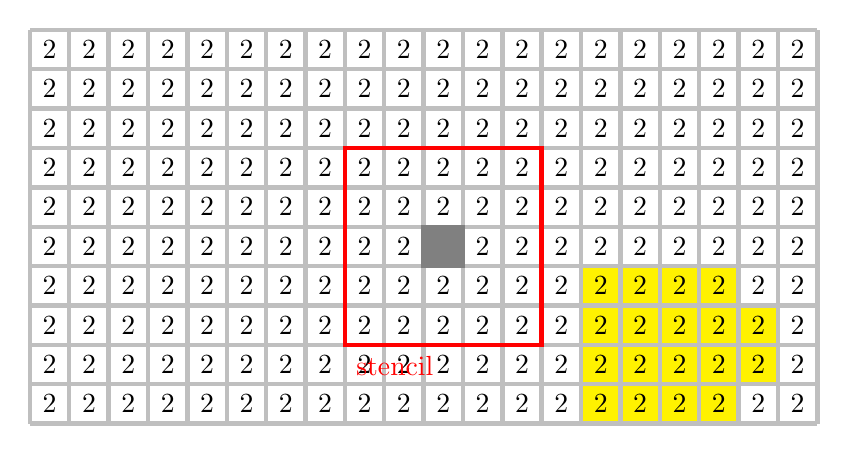
\begin{tikzpicture}[scale=0.5,ultra thick]
        % Define grid dimensions
        \def\nRows{10}
        \def\nCols{20}
        \pgfmathsetmacro\nRowsm{\nRows-1}
        \pgfmathsetmacro\nColsm{\nCols-1}

        \foreach \row in {0,...,\nRowsm} {
            \foreach \col in {0,...,\nColsm} {
                \pgfmathsetmacro\distance{veclen(\col-4.356, \row-2.65)};
                \pgfmathparse{\distance < 4 ? "blue" : "white"}
                \edef\colour{\pgfmathresult};
                \ifthenelse{\equal{\colour}{blue}}{                    
                    \fill[\colour!60!white] (\col, \row) rectangle ++(1,1);
                    \node (num) at (\col +0.5,\row+0.5){1};
                }
            }
        }

        \foreach \row in {0,...,\nRowsm} {
            \foreach \col in {0,...,\nColsm} {
                \pgfmathsetmacro\distance{veclen(\col-15, \row-6.2)};
                \pgfmathparse{\distance < 3.5 ? "blue" :"white"}
                \edef\colour{\pgfmathresult};
                \ifthenelse{\equal{\colour}{blue}}{
                    \fill[\colour!60!white] (\col, \row) rectangle ++(1,1);
                \node (num) at (\col +0.5,\row+0.5){2};
                }
            }
        }

        \foreach \row in {0,...,\nRowsm} {
            \foreach \col in {0,...,\nColsm} {
                \pgfmathsetmacro\distance{veclen(\col-15.62, \row-1.5)};
                \pgfmathparse{\distance < 2.5 ? "yellow" :"white"}
                \edef\colour{\pgfmathresult};
                \ifthenelse{\equal{\colour}{yellow}}{
                    \fill[\colour] (\col, \row) rectangle ++(1,1);
                    \node (num) at (\col +0.5,\row+0.5){2};
                }
            }
        }
        % Define grid size
        \pgfmathsetmacro\gridSize{1}
        
        \foreach \row in {0,...,\nRows} {
            \draw [gray!50] (0,\row*\gridSize) -- (\nCols*\gridSize,\row*\gridSize);
        }
        % Draw vertical grid lines
        \foreach \col in {0,...,\nCols} {
            \draw [gray!50] (\col*\gridSize,0) -- (\col*\gridSize,\nRows*\gridSize);
        }
        % Draw drop shape
        \draw[red] (8,2)node[below right]{stencil} rectangle +(5,5); % Draw the rectangular base
        \filldraw[gray] (10,4) rectangle +(1,1);
    \end{tikzpicture}    
    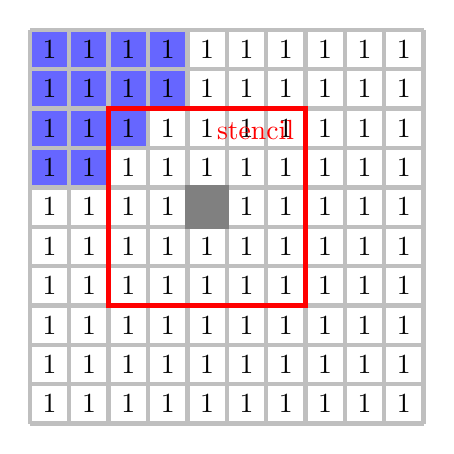
\begin{tikzpicture}[scale=0.5,ultra thick]
        % Define grid dimensions
        \def\nRows{10}
        \def\nCols{10}
        \pgfmathsetmacro\nRowsm{\nRows-1}
        \pgfmathsetmacro\nColsm{\nCols-1}

        \foreach \row in {0,...,\nRowsm} {
            \foreach \col in {0,...,\nColsm} {
                \pgfmathsetmacro\distance{veclen(\col, \row-2)};
                \pgfmathparse{\distance < 3.5 ? "blue" :"white"}
                \edef\colour{\pgfmathresult};
                \ifthenelse{\equal{\colour}{blue}}{
                    \fill[\colour!60!white] (\col, \row) rectangle ++(1,1);
                \node (num) at (\col +0.5,\row+0.5){1};
                }
            }
        }

        \foreach \row in {0,...,\nRowsm} {
            \foreach \col in {0,...,\nColsm} {
                \pgfmathsetmacro\distance{veclen(\col-7, \row-2)};
                \pgfmathparse{\distance < 3.5 ? "blue" :"white"}
                \edef\colour{\pgfmathresult};
                \ifthenelse{\equal{\colour}{blue}}{
                    \fill[\colour!60!white] (\col, \row) rectangle ++(1,1);
                    \node (num) at (\col +0.5,\row+0.5){1};
                }
            }
        }
        \foreach \row in {0,...,\nRowsm} {
            \foreach \col in {0,...,\nColsm} {
                \pgfmathsetmacro\distance{veclen(\col-5, \row)};
                \pgfmathparse{\distance < 3.5 ? "blue" :"white"}
                \edef\colour{\pgfmathresult};
                \ifthenelse{\equal{\colour}{blue}}{
                    \fill[\colour!60!white] (\col, \row) rectangle ++(1,1);
                    \node (num) at (\col +0.5,\row+0.5){1};
                }
            }
        }
        \foreach \row in {0,...,\nRowsm} {
            \foreach \col in {0,...,\nColsm} {
                \pgfmathsetmacro\distance{veclen(\col, \row-9)};
                \pgfmathparse{\distance < 3.5 ? "blue" :"white"}
                \edef\colour{\pgfmathresult};
                \ifthenelse{\equal{\colour}{blue}}{
                    \fill[\colour!60!white] (\col, \row) rectangle ++(1,1);
                    \node (num) at (\col +0.5,\row+0.5){1};
                }
            }
        }
        % Define grid size
        \pgfmathsetmacro\gridSize{1}
        
        \foreach \row in {0,...,\nRows} {
            \draw [gray!50] (0,\row*\gridSize) -- (\nCols*\gridSize,\row*\gridSize);
        }
        % Draw vertical grid lines
        \foreach \col in {0,...,\nCols} {
            \draw [gray!50] (\col*\gridSize,0) -- (\col*\gridSize,\nRows*\gridSize);
        }
        % Draw drop shape
        \draw[red] (2,3) rectangle +(5,5)node[below left]{stencil}; % Draw the rectangular base
        \filldraw[gray] (4,5) rectangle +(1,1);
    \end{tikzpicture}    
    \caption{Sketch of two situations were the \textit{near contact} criterion is true. 
    The background grid represents the cells within the numerical domain. 
    The dark blue area represents the cells where $C_i > 0$.
    The yellow area represents the cells where the tracer $C_j > 0$ for $j\neq i$. 
    The numbers represent the values of the $Tag$ scalar field within each tracer.
    The $5$ by $5$ cells red rectangle represents the stencil zone which iterates over all cells of the domain.  
    %  where the center of the stencil (gray square) must respect $C_i = 0$. 
    (left) Two droplets in contact since we have two opposite cells in the stencil with $C_i > 0$ and $C_i=0$ at the center.
    And the mentioned cells belong to two different regions so that (\textit{Step 3}) is also validated.  
    (right) A near contact is observed since we have two opposite cells in the stencil with $C_i > 0$ and $C_i=0$ at the center, however in this case we do not verify the second criterion of \textit{Step 3} which requires two different tags values. 
    }
    \label{fig:criterion}
\end{figure}
These four steps are executed at each simulation time step and for each tracer $C_i$ with $i = 1, 2, \ldots, N(t)$.
Following this procedure, we ensure that all adjacent droplets are using different tracers, which ultimately prevents coalescence. 

Having $N(t)$ tracers requires some modifications to the aforementioned governing equations. 
Specifically, instead of solving \ref{eq:dt_C}, we solve $N(t)$ transport equations, one for each $C_i$.
Likewise, the surface tension force is computed as the sum of the contributions from each $C_i$ and reads
\begin{align*}
    \pddt C_i + \textbf{u}\cdot\grad C_i = 0,
    \ \  \ \ \forall i = 1,2,\ldots N(t),\\
    \textbf{f}_\gamma 
    = \sum_{i=0}^{N(t)} \gamma \kappa_i \grad C_i
\end{align*}
where $\kappa_i$ is the numerical approximation of the curvature of the interface of field $C_i$, which is computed following the same method employed for a single tracer. 

\ref{fig:diagram} (left) shows a snapshot of a simulation at an arbitrary time $t^* = 100 \sqrt{g/d}$. 
The droplet interfaces are colored by the indices of their respective tracer. 
In this simulation at that time, no more than 3 colors are needed to avoid coalescence.
On \ref{fig:diagram} (right) we display the value of $N(t)$ in term of the dimensionless simulation time for various volume fractions $\phi$ at $Ga = 50$ and  $\lambda = 1$. 
We observe that for the entire simulation, no more than 3 tracers were needed for the dilute emulsion ($\phi = 0.01$) and up to 7 for the denser regime ($\phi = 0.2$). 
Although our algorithm might not be optimized, it brings sufficient efficiency for our needs. 
Indeed, \ref{tab:performance} reports the time spent by each function during a simulation. 
It is observed that the \texttt{no-coalesce.h} algorithm accounts for approximately $4\%$ of the total computational time of a simulation. 
As for the \texttt{tag.h} algorithm, its cost is around $2\%$, which is also reasonable.
In comparison, the \texttt{poisson.h} solver is about $13\%$ of the simulation time. 
The advection of VoF tracers is about $7\%$ which is relatively high but still reasonable.
To reduce the cost related to the \texttt{no-coalesce.h} algorithm we believe that further developments, which are referenced at \href{http://basilisk.fr/sandbox/fintzin/Rising-Suspenion/no-coalescence.h}{no-coalescence.h}, are still doable and could be useful for future studies.
\begin{figure}[h!]
    \centering
    \begin{tikzpicture}
    \node (img) at (0,0) {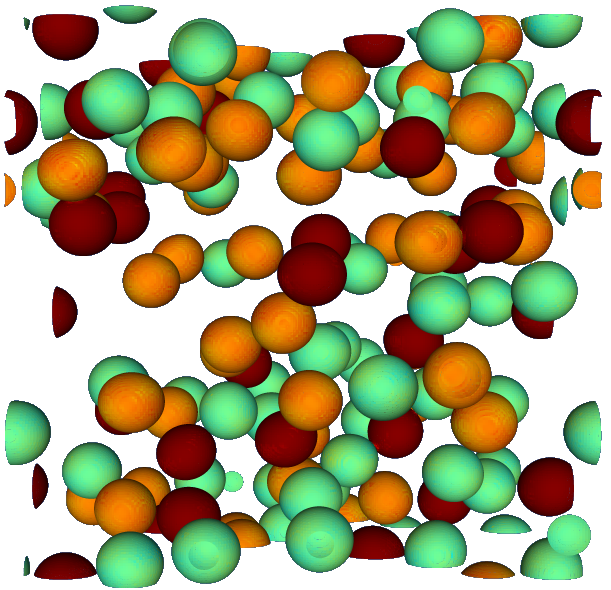
\includegraphics[width = 0.4\textwidth]{image/VoF2.png}};
    \node (img) at (0.4\textwidth,-0.01\textwidth) {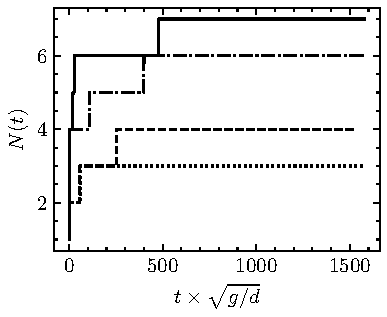
\includegraphics[width = 0.4\textwidth]{image/HOMOGENEOUS_NEW/CA/NVoF_vs_t_Ga_50_l_1.pdf}};
    \end{tikzpicture}
    \caption{
    (left) Snapshot of a DNS with $\phi = 0.05$, $\lambda = 1$, $Ga = 50$ with the interface of the droplets colored by the index of the tracers.
    (right) Number of tracers $N(t)$ as a function the dimensionless time.
    Four different volume fractions are displayed : (dotted line) $\phi = 0.01$, (dashed line) $\phi = 0.05$ (dash dotted line) $\phi = 0.1$ (solid line) $\phi = 0.2$ at $Ga = 50$ and $\lambda = 1$. 
    }
    \label{fig:diagram}
\end{figure}


In order to validate our numerical methodology, we have compared our numerical results to the experiments of \citet{mohamed2003drop} where they experimentally study the impact of a single drop on a flat interface of the same fluid. %, while recording the positions of the interfaces.
It is found that the multi-VoF method captures remarkably well the position of interfaces, even with a poor description of the liquid film between these interfaces.
Additionally, we argue that the mesh independence study conducted in \ref{ap:validation} (Case 3) substantiates the accuracy of the DNS, as the dynamics of interaction do converge with  reasonable errors for a grid resolution of $\Delta/d = 30$. 
Overall, we used an optimized multi-VoF method, enabling us to perform DNS with a maximum of 7 tracers in the densest scenario.
 







\section{Nearest particle statistics}
\label{sec:nearest}

To study the emulsions' microstructure, we chose to adopt the \textit{nearest particle statistics} framework recently revisited by \citet{zhang2021ensemble}.
We now recall some definitions of the \textit{nearest particle statistics} averaging procedure. 
For further details, readers are encouraged to refer to \citet{zhang2023evolution} on which this work mostly relies.

\subsubsection*{Theoretical framework}
Let $P(\FF)$ be the probability density function that describes the probability of finding the flow in the configuration $\FF$, where $\FF = (\lambda_1,\lambda_2,\lambda_3,\ldots)$ is a finite set of all the parameters describing the initial flow configuration.
% \footnote{We assume that the flow can be described by a finite number of parameters related to both phase.}. 
Then, we define $d\mathscr{P} = P(\FF)d\FF$ as the probable number of realizations in the incremental region of the flow' phase space, $d\FF$ around $\FF$.
Additionally,  $\textbf{x}_i(t,\FF)$ and $\textbf{x}_j(\FF,t)$ refers to the Lagrangian position vectors of the particles $i$ and $j$, respectively. 
We also introduce the age of the interaction, denoted as $a$, which represents the time elapsed since two particles became nearest neighbors.
Then, the nearest pair probability density function is given by,
\begin{equation}
    P_{nst}(\textbf{x},\textbf{r},a,t)= 
    \int \sum_{i}^{N_b}\delta(\textbf{x}-\textbf{x}_i)
    \sum_{j\neq i}^{N_b}\delta(\textbf{x}+\textbf{r}-\textbf{x}_j) 
    \delta(t+a-t_c^{ij}) 
    h_{ij} d\mathscr{P},
    \label{eq:P_nstij}
\end{equation}
where we introduced the function $h_{ij}$, which equals $1$ if and only if particle $j$ is one of the nearest neighbors of particle $i$, and $h_{ij} = 0$ otherwise. 
$t_c^{ij}(\FF,t)$ represents the time at which particles $i$ and $j$ became nearest neighbors. 
Formally, we have $a = t - t^{ij}_c(\FF,t)$.
Consequently, $P_{nst}(\textbf{x},\textbf{r},t,a)$ is the probability of having a particle center of mass located at $\textbf{x}$ at time $t$ with it nearest neighbor at $\textbf{x}+\textbf{r}$ given that the pair of particles have been nearest neighbors since $a$ time.
Note that $P_\text{nst}(\textbf{x},\textbf{r},t,a)$ is related to the number density $n_p(\textbf{x},t)$ through the relationship, 
\begin{equation*}
    \int_0^\infty 
    \int_{\mathbb{R}^3}
     P_\text{nst}(\textbf{x},\textbf{r},t,a) d\textbf{r} da = n_p(\textbf{x},t). 
    \label{eq:Pnst}
\end{equation*}
This establishes consistency between the nearest particle statistic and kinetic theory. 


Furthermore, $\textbf{w}_{ij}(t,\FF) = \textbf{u}_j(t,\FF) - \textbf{u}_i(t,\FF)$ represents the relative velocity between the particles $i$ and $j$, at time $t$ in the configuration $\FF$. 
With, $\textbf{u}_i(t,\FF)$ and $\textbf{u}_j(t,\FF)$, the Lagrangian center of mass velocities of the particles $i$ and $j$, respectively. 
The formal expression of the ensemble average of such a quantity is given by,
\begin{equation*}
    \textbf{w}^\text{nst}_p P_{nst}(\textbf{x},\textbf{r},t,a)
    = 
    \int \sum_{i}^{N_b}\delta(\textbf{x}-\textbf{x}_i)
    \sum_{j\neq i}^{N_b}\delta(\textbf{x}+\textbf{r}-\textbf{x}_j) 
    \delta(t+a-t_c^{ij}) 
    \textbf{w}_{ij}
    h_{ij} 
    d\mathscr{P}.
    \label{eq:q_nstij}
\end{equation*}
Following this definition, $\textbf{w}^\text{nst}_p(\textbf{x},\textbf{r},t,a)$ is the averaged relative velocity between the nearest pairs, conditioned on the presence of a particle at $\textbf{x}$ and time $t$, with its nearest neighbor at $\textbf{x}+\textbf{r}$ with age $a$. 
The physical meaning of such a field will be further investigated in \ref{sec:velocity}. 
The superscript $^\text{nst}$ indicates that $\textbf{w}_{ij}(\FF,t)$ is ensemble-averaged conditionally on the presence of the nearest neighbor, and the subscript $_p$ indicates that it is at the origin a Lagrangian property. 
More generally, $\textbf{w}_{ij}(t,\FF)$ can be replaced by any particle properties, an example used in this work is $\textbf{u}_i(\FF,t)$.
In this case, $\textbf{u}^\text{nst}_p(\textbf{x},\textbf{r},t,a)$ represents the conditionally-averaged particle phase velocity, given the presence of a particle at \textbf{x} and time $t$, with its nearest neighbor position at $\textbf{x}+\textbf{r}$ with age $a$. 

Since, we model a statistically steady and homogeneous configuration, the variables $\mathbf{x}$ and $t$ seem to have no interest. 
Nevertheless, we argue that $\mathbf{x}$ and $t$ indicate the dependence of the averaged quantities on the global flow parameters, $Ga$, $\phi$, $Bo$, $\zeta$, and $\lambda$.
Therefore, it is essential to retain $\mathbf{x}$ and $t$ in our notation. 



\subsubsection*{Numerical sampling}

To reconstruct all these statistics from the DNS, we treat each simulation time step  as an independent flow configuration, denoted as, $\FF$. 
Under this assumption, the ensemble average operators can be rewritten as :
\begin{equation}
    \int  d\PP\ldots
    = \frac{1}{E}\sum_\FF^\text{E} \ldots 
    \label{eq:discrete_ensemble_average}
\end{equation}
where $E$ is the total number of events, which, in our case, corresponds to the total number of time steps simulated.  
When performing conditional average based on the position of the nearest neighboring particle, the methodology is slightly different. 
To reconstruct a quantity such as $\textbf{w}^\text{nst}_p(\textbf{x},\textbf{r},t,a)$ we gather all the relative velocity $\textbf{w}_{ij}(t;\FF)$ from the simulation and store them in $n$ intervals of ages $\Delta a_k$, and relative positions $\Delta \textbf{r}_k$ for $k = 1,\ldots, n$.
Then, we apply the discrete ensemble average on $\textbf{w}_{ij}(t;\FF)$ for each group independently.
Formally, we write, 
\begin{equation}
    \textbf{w}^\text{nst}_p(\textbf{x},t,\Delta\textbf{r}_k,\Delta a_k)
    = \frac{1}{E_k} 
    \sum^{E_k}_{\FF_k} 
    % \sum_i^{N_b}
    % \sum_{j\neq i}^{N_b}
    \textbf{w}_{ij}(t;\FF_k)
    % h_{ij}
    % \text{\;\;  with  \;\;}
    % \FF_k = \{\FF; \textbf{r}(\FF)\in\Delta \textbf{r}_k, a(\FF)\in  \Delta a_k\}
    \label{eq:vec_cond}
\end{equation}
where $\FF_k$ correspond to the events were the nearest particle pair $i$ and $j$ respects $\textbf{r},a \in \Delta \textbf{r}_k ,\Delta a_k$.
$E_k$ is the total number of events fulfilling these constraints. 
Finally, we obtained an approximation of $\textbf{w}^\text{nst}_p(\textbf{x},\textbf{r},t,a)$ which takes the intervals, $(\Delta\textbf{r}_i,\Delta a_i)$ as input.
At some point, it will be useful to study the averaged relative velocity, conditioned on the age or on the radial distance, independently. 
Therefore, in a more general way if $p$ is a scalar property with $\Delta p_k$ its $n$ intervals, we can define the $p$-conditionally averaged relative velocity as, 
\begin{equation}
    \textbf{w}^\text{nst}_p(\textbf{x},t,\Delta p_k)
    = \frac{1}{E_{k}} 
    \sum^{E_{k}}_{\FF_{k}}  
    % \sum_i^{N_b} 
    % \sum_{j\neq i}^{N_b}
    \textbf{w}_{ij}(t;\FF_k)
    % h_{ij}
    % \text{\;\;  with  \;\;}
    % \FF_k = \{\FF; p(\FF)\in\Delta p_k\}
    \label{eq:scalar_cond}
\end{equation}
In this definition, $\FF_{k}$ corresponds to all the events where the nearest pair $i$ and $j$ respect the condition, $p \in \Delta p_k$, and $E_{k}$ represents the total number of events where $p\in\Delta p_k$. 

It is clear that to obtain representative averaged quantities, the number of events $E_k$ per intervals must be consequent. 
For 2D-conditioned quantity such as \ref{eq:vec_cond}, we estimated that $100$ samples per bins were sufficient to obtain qualitative results. 
Consequently, the plots exposed in \ref{sec:velocity} have been generated by averaging the quantity of interest (velocity fields, age of interaction) with a minimum threshold of $E_k = 100$ samples for each bin.
Regarding the scalar-conditioned fields such as in \ref{eq:scalar_cond}, we gathered $E_k = 1000$ sample per bins to obtain an accurate and quantitative results. 
Lastly, regarding the sampling, we collected data for each Lagrangian quantity every $10$ simulation time steps. 
The simulation time step is determined either by a Courant Friedrichs Lewy (CFL) condition or by the capillary time step, depending on the dimensionless numbers involved.
On average, $200,000$ time steps are performed during a simulation with $N_b = 125$ droplets. This results in a total number of $E = 2,500,000$ samples. In \ref{ap:validation} (\textit{Case 3}), we demonstrate that our statistics are well-converged.



\section{Microstructure}
\label{sec:microstructure}
This section presents an analysis of the microstructure based on the nearest neighbor probability density function. 
%age included nearest pair probability density function  $P_\text{nst}(\textbf{x},\textbf{r},t,a)$ and on .


%After identifying the different forms of the microstructure with respect to the dimensionless parameters, we introduce a general and concise way to quantify it.
By definition, $P_\text{nst}(\textbf{r}|\textbf{x},t)$ does not require symmetry with respect to the variable $\textbf{x}+\textbf{r}$ and \textbf{x}, as is the case for classical particle-pair distribution functions. 
Nevertheless, it turns out that $P_\text{nst}$ possesses a nearly-symmetric distribution, such that  $P_\text{nst}(r,\theta)\approx P_\text{nst}(r,- \theta)$ as demontrated below.
\begin{figure}[h!]
    \centering
    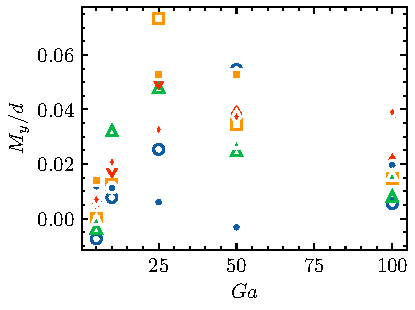
\includegraphics[height = 0.3\textwidth]{image/HOMOGENEOUS_NEW/PA/Ry.pdf}
    \caption{ Dimensionless first moment of the nearest particle pair distribution in the direction of gravity $M_y/d$. 
    ($\pmb\bigcirc$) $\phi = 0.01$; ($\pmb\triangle$) $ \phi = 0.05$; ($\pmb\square$) $\phi = 0.1$ ($\pmb\lozenge$) $\phi = 0.2$.
    The hollow symbols correspond to $\lambda = 1$, the filled symbols to $\lambda = 10$.
    % For $r<d$ we arbitrarily set $P_\text{r}^\text{th} = 1$ so that the distribution can be visualized.
    % Black symbols represent the results of \citet{zhang2023evolution} for hard sphere suspension with $\phi = 0.016,0.056,0.134,0.262$  %$\phi = 0.0168,0.0565,0.1341,0.2622$ 
    % corresponding to $\pmb\times,\pmb +, \pmb\star , \pmb\triangledown$, respectively.
    }
    \label{fig:ap:RY}
\end{figure}
%This is demonstrated by \ref{fig:ap:RY} 
%where we can see that the first moment of $P_\text{nst}$, namely
We define the first moment of $P_\text{nst}$ as
\begin{equation}
 \textbf{M} = \int_{\mathbb{R}^3} \textbf{r} P_\text{nst}(\textbf{r}) d\textbf{r}.
\end{equation}
\ref{fig:ap:RY} illustrates the projection of $\textbf{M}$ along the direction of gravity. 
The relatively small but finite values of $M_y$ indicate that $P_\text{nst}$ exhibits a nearly symmetric distribution with respect to $\theta$.
Nevertheless, this indicates that the nearest neighbor is more likely to be located in the upstream direction. 
Note that this is consistent with the findings of \citet{zhang2023evolution}.
Even though this slight asymmetry might have its importance \cite{zhang2023evolution}, we discard it in this study. 
Therefore, we choose to show only the upper part of the distribution in the following plots, (displayed in \ref{fig:Pnst_low_Ga} and \ref{fig:Pnst_high_Ga}) since qualitatively it remains the same as the lower part.  
Additionally, in the discussion below, we refer to the sphere at the origin of the graphs, located at $\textbf{x}=0$, as the \textit{test particle}.%\textit{test particle} or the \textit{test particle}. 

\subsection{Low inertia regimes}
We begin with a detailed analysis of $P_\text{nst}$ at $Ga =10$, to investigate the influence of $\lambda$ and $\phi$ on the microstructure when inertial effects are small.
\begin{figure}[h!]
    \centering
    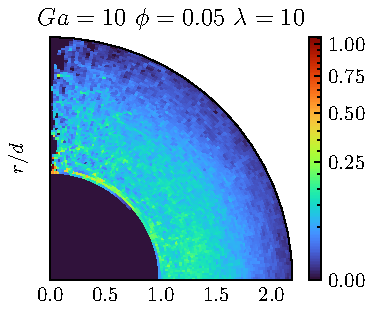
\includegraphics[height=0.21\textwidth]{image/HOMOGENEOUS_NEW/Dist/Pnst_l_10_Ga_10_PHI_0_05.pdf}
    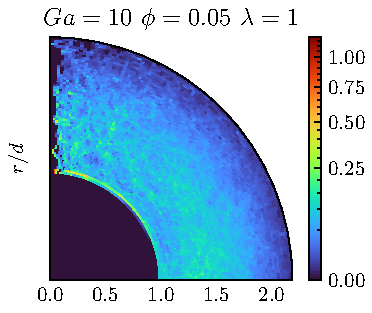
\includegraphics[height=0.21\textwidth]{image/HOMOGENEOUS_NEW/Dist/Pnst_l_1_Ga_10_PHI_0_05.pdf}
    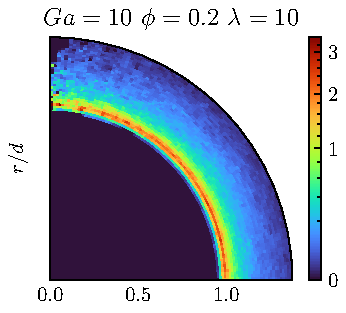
\includegraphics[height=0.21\textwidth]{image/HOMOGENEOUS_NEW/Dist/Pnst_l_10_Ga_10_PHI_0_2.pdf}
    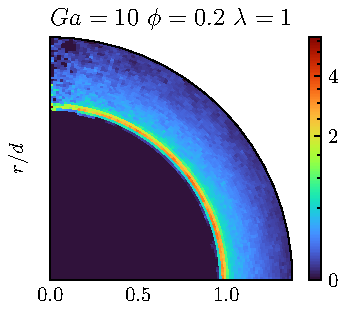
\includegraphics[height=0.21\textwidth]{image/HOMOGENEOUS_NEW/Dist/Pnst_l_1_Ga_10_PHI_0_2.pdf}
    \caption{Histogram of the probability density function, $P_\text{nst}(r,\theta)$, for low inertia $Ga = 10$.
    The color map represents the nearest pair distribution function. %the values of $P_\text{nst}$.
    The origin corresponds to the position of the \textit{test particle}.
    The dimensionless radial and azimuthal coordinates, $|\textbf{r}|/d$ and $\theta$, correspond to the nearest neighbor position.
    The vertical direction corresponds to the flow direction, which is also the axis of symmetry for $P_\text{nst}$.
    (left) Low volume fraction cases $\phi=0.05$ for $\lambda = 1,10$.
    (right) High volume fraction cases $\phi=0.2$ for $\lambda = 1,10$.
    }
    \label{fig:Pnst_low_Ga}
\end{figure}
The first observation from \ref{fig:Pnst_low_Ga} indicates that the likelihood of finding the nearest neighboring particle at an angle $\theta$ is uniform across all $\theta$.
This suggests that $P_\text{nst}$ is isotropic at these \textit{Galileo} numbers. We can observe that $P_\text{nst}$ is larger close to the \textit{test particle} ($r/d = 1$) in the high volume fraction cases than in the low volume fraction cases.
%If we compare the low volume fraction cases to the high volume fraction cases, we can observe that $P_\text{nst}$ is larger at near contact of the test particle ($r/d = 1$) in the latter case.
% For solid particles it is also common that pair distributions are more concentrated at the contact of the test particle for increasing $\phi$. 
In practice, if particles are more likely to be close to one another, it means that densely packed regions of particles are present in the flow.
This suggests that isotropic clusters, as represented in \ref{fig:scheme_clusters} (\textit{Case 2}), are likely to form in the present context. 
Regarding the effect of the viscosity ratio, $P_\text{nst}$ are very similar for both values of $\lambda$ except that for the highest volume fraction the region of highest probability is thinner for the lowest aspect ratio. 
Consequently, in this regime we find homogeneous microstructures at low $\phi$, and non-homogeneous but still isotropic microstructure (\textit{``clusters''}) at higher $\phi$. 


\subsection{High inertia regimes }
We now focus on the high inertia regimes ($Ga =80$).
In this situation, it is expected that the presence of particle wakes modify the interactions between particles \citep{yin2007}. 
\begin{figure}[h!]
    \centering
    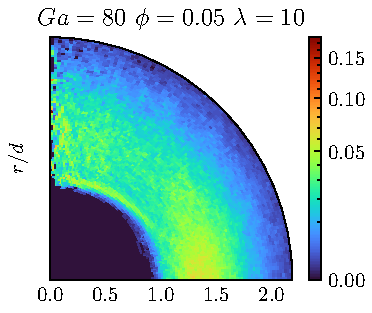
\includegraphics[height=0.205\textwidth]{image/HOMOGENEOUS_final/Dist/Pnst_l_10_Ga_80_PHI_0_05.pdf}
    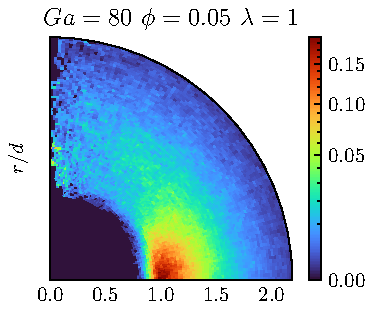
\includegraphics[height=0.205\textwidth]{image/HOMOGENEOUS_final/Dist/Pnst_l_1_Ga_80_PHI_0_05.pdf}
    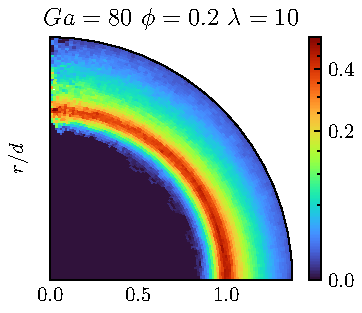
\includegraphics[height=0.205\textwidth]{image/HOMOGENEOUS_final/Dist/Pnst_l_10_Ga_80_PHI_0_2.pdf}
    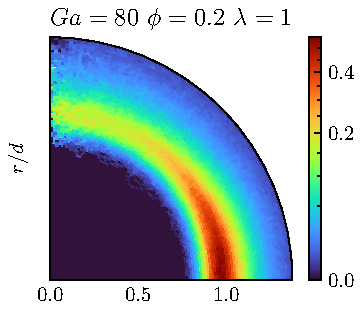
\includegraphics[height=0.205\textwidth]{image/HOMOGENEOUS_final/Dist/Pnst_l_1_Ga_80_PHI_0_2.pdf}
    \caption{Histogram of the normalized function $P_\text{nst}$ at high inertia $Ga = 80$.
    The color map represents the values of the nearest pair distribution function. %of $P_\text{nst}$.
    The origin corresponds to the position of the \textit{\textit{test particle}}.
    The dimensionless radial and azimuthal coordinates, $|\textbf{r}|/d$ and $\theta$, correspond to the nearest neighbor position.
    The vertical direction corresponds to the flow direction, which is also the axis of symmetry for $P_\text{nst}$.
    (left) Low volume fraction cases $\phi=0.05$ for $\lambda = 1,10$.
    (right) High volume fraction cases $\phi=0.2$ for $\lambda = 1,10$.}
    \label{fig:Pnst_high_Ga}
\end{figure}
%If we compare \ref{fig:Pnst_high_Ga} (right) with their counterparts from \ref{fig:Pnst_low_Ga} (right) we observe that $P^n_\text{r}$ becomes even larger at contact of the particles for $Ga=80$.
%Again, this could witness of the presence of clustering of particles. 
%In general, all $P_\text{nst}$ from \ref{fig:Pnst_high_Ga} exhibit some differences compared to the cases \ref{fig:Pnst_low_Ga}. 
%In the high inertial cases (\ref{fig:Pnst_high_Ga}), we can notice that $P_\text{nst}$ is larger on the sides of the \textit{test particle} for the iso-viscous emulsions ($\lambda = 1$).
Anisotropy in \ref{fig:Pnst_high_Ga} for $\lambda=1$ is particularly striking compared to \ref{fig:Pnst_low_Ga}. 
In the former, a higher concentration of particles is identified at $\theta \approx 0$, as seen in \ref{fig:Pnst_high_Ga}. 
A higher concentration of $P_\text{nst}$ around $\theta \approx 0$ indicates the presence of horizontal rafts of particles. 
In this case, the microstructure is non-homogeneous and anisotropic; this situation is illustrated in \ref{fig:scheme_clusters} (\textit{Case 3: ``layers''}). 
As the \textit{Galileo} number ($Ga$) increases and for low values of the viscosity ratio ($\lambda$), the probability of having neighbors on the horizontal plane of the \textit{test particle} increases. 
This leads to an increase in the anisotropy of the microstructure, which is more pronounced for low volume fractions. 
In contrast, the high-viscosity drops display an isotropic distribution of the nearest particles around the \textit{test particle}. 
This observation suggests the presence of isotropic clustering of particles.


%In comparison the high viscosity drops show an isotropic discitrbution of nearest particle around the \textit{test particle}. This could witness of the presence of isotropic clustering of particles.

%We do not observe a significant effect of the volume fraction on the anisotropy of the distribution.
%However, at this stage it remains unclear if increasing $\phi$ have a positive or negative impact on the anisotropy of the distribution. 

To illustrate the impact of $\lambda$ on the microstructure, \ref{fig:images} displays snapshots of two DNS at $\phi = 0.05$ and $Ga = 80$. 
As predicted by $P_\text{nst}$, we observe layers and particles in close contact for $\lambda = 1$, contrasting with the seemingly more evenly dispersed microstructure for $\lambda = 10$.
\begin{figure}[h!]
   \centering
   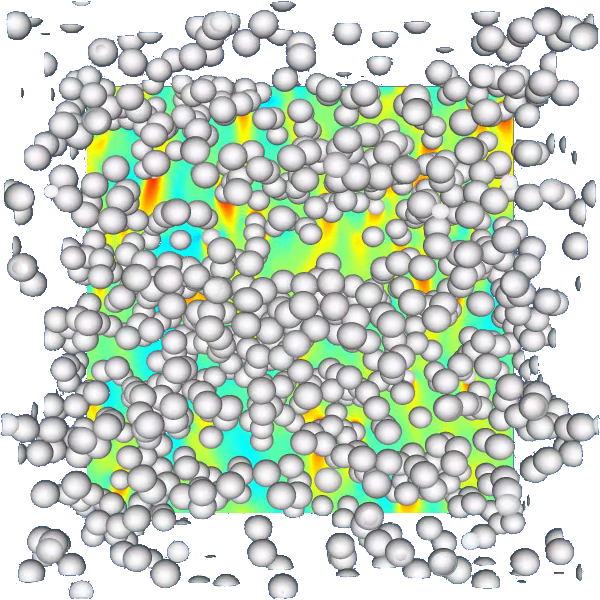
\includegraphics[width=0.45\textwidth]{image/HOMOGENEOUS_final/Ga_80_phi_005_l_1.png}
   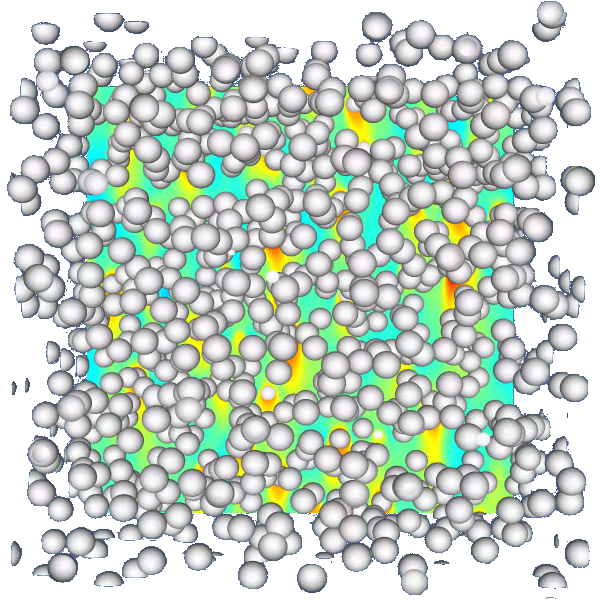
\includegraphics[width=0.45\textwidth]{image/HOMOGENEOUS_final/Ga_80_phi_005_l_10.png}
   \caption{Snapshot of a simulation at $t^* = 200$ for $\phi=0.05$ and $Ga=80$.
   Color map : values of the vertical component of the velocity, field on the vertical plane defined by the equation $z=0$. 
   (left)  $\lambda = 1$.
   (right)  $\lambda = 10$.
   }
   \label{fig:images}
\end{figure}
In fact, for $\lambda = 10$, in \ref{fig:images} (right), we can still observe horizontal rafts of droplets or droplets rising side-by-side, but this effect is not as pronounced as for $\lambda = 1$. 
Drops with high viscosity ratios maintain a significant distance between other drops, which prevents the creation of structures such as droplet layers.
% This might be because of a higher vorticity around the viscous droplets.   
% As discussed in \citet{zhang2021three}, rising pairs of spherical bubbles may reach a stable side-by-side configuration, which tends to generate horizontal clusters.
% They range of dimensionless parameters is consistent with the ones presented in this study, making this hypothesis valuable for iso-viscous emulsions. 
% In \citet{legendre2003hydrodynamic} they study the interaction of a bubble pair rising side-by-side. 
% They stipulate that for two bubbles at moderate \textit{Reynolds} number $50-100$, the interaction forces are found to be repulsive, while it is attractive or null for higher \textit{Reynolds} number. 
% In our case it is reasonable to think that such pair attraction / repulsion mechanisms might drive the clustering mechanism.
%On another note, we can observe on \ref{fig:images} (left) that the distance between the layers is roughly equal to the length of the numerical domain. 
%Indeed, only one layer of droplets is present in the domain. 
%Therefore, the current microstructure is constrained by the size of the numerical domain, it is probably not representative of the real microstructure that we would obtain in an infinite non-periodic domain. 
%Additionally, one might argue that the layers appear due to collective effects drove by the size of the box.
%Indeed, it is exactly what we observe for small number of bubbles ($N_b = 4$) rising in a periodic domain, see \citet{loisy2017}. 
%However, we might expect that horizontal layers such as the one observed in \ref{fig:images} (left) still remain for lager boxes since the number of droplets is consequent.
%In our case, the presence of horizontal raft might be the consequence of pairwise interactions mechanism, as discussed above. 
%Therefore, it is likely that that layers still appear regardless of the size of the box.
%Nevertheless, the distance between these layers is still constrained by the size of the numerical domain, despite the consequent number of droplets used here. 
%In all rigor, DNS in a larger domain with more particles would be required to evaluate the microstructure dependence on the domain size. 
%Nevertheless, due to evident numerical constrains it has not been performed in this study.  
From the present analysis of $P_\text{nst}$ and the actual microstructure presented in \ref{fig:images} we can infer that the \textit{nearest particle statistics} is able to predict features in the microstructure such as layers and clusters. 


\subsection{Nearest particle radial distribution function }

Although \ref{fig:Pnst_low_Ga} and \ref{fig:Pnst_high_Ga} give a good qualitative representation of the particle-pair azimuthal distribution, they fall short in delivering a quantitative depiction of the radial distribution.
Thus, in this section we investigate the value of the radial distribution function $P_\text{r-nst}$ defined in \ref{eq:P_r}. 
For a random isotropic distribution of hard spheres, it is possible to derive a theoretical prediction for $P_\text{nst}$ obtained in the vanishing volume fraction limit. 
Indeed, it is shown in \citet{zhang2021ensemble} that for a dilute random arrangement of particles $P_\text{nst}(r)$, reads as
\begin{equation}
    P_\text{nst}^{\phi \ll 1}(r) = n_p e^{- 8\phi\left[(r/d)^3-1\right]}.
    \label{eq:Pnst_dilute}
\end{equation}
It must be understood that this formula is accurate only at $\mathcal{O}(\phi)$; therefore, in most cases, it is not expected to be representative.
Additionally, \citet{torquato1990nearest} derived a radial distribution function for hard spheres at arbitrary volume fractions $\phi$. In our notation, this distribution can be written
\begin{equation}
    P_\text{nst}^\text{th}(r) = 
        n_p\left(e+\frac{f}{(r/d)} +\frac{g}{(r/d)^2}\right)
    e^{-\phi\left[8e\left((r/d)^3-1\right)+12 f\left((r/d)^2-1\right)+24g\left((r/d)-1\right)\right]}
    \label{eq:torquato}
\end{equation}
with, 
\begin{align*}
    && e= \frac{1+\phi}{(1-\phi)^3},
    && f= \frac{-\phi (3+\phi)}{2(1-\phi)^3},
    && g= \frac{\phi^2}{2(1-\phi)^3}.
\end{align*}
\begin{figure}
    \centering
    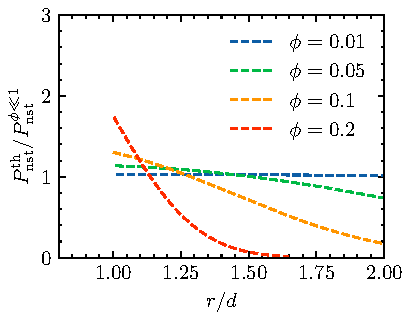
\includegraphics[height=0.3\textwidth]{image/HOMOGENEOUS_final/Dist/Theory.pdf}
    \caption{
        Theoretical prediction of $P_\text{nst}^{th}/P_\text{nst}^{\phi \ll 1}$ in terms of the dimensionless distance $r/d$ for four volume fraction $\phi$. 
    }
    \label{fig:torquato}
\end{figure}
%In both cases 
In \ref{fig:torquato} we show that $P_\text{nst}^\text{th}(r)$ predict a more concentrated nearest neighbor concentration at the contact of the \textit{test particle} ($r/d=1$) compared to the dilute random distribution $P_\text{nst}^{\phi\ll 1}(r)$. 
This effect is solely due to the consideration of the impenetrability of hard spheres. 
It should be noted that both \ref{eq:Pnst_dilute} and \ref{eq:torquato} do not consider the influence of the surrounding fluid nor the deformation of particles. 
%and may differs %from the droplet pair distribution.
In particular, for hard sphere $P_\text{nst}^\text{th} = 0$ for $r<d$ while in our case, particles might deform at contact, meaning that $P_\text{r-nst}$ is finite for certain $r<d$. 
However, using these theoretical probability density functions for comparative purposes remains valuable. 


\begin{figure}[h!]
    \centering
    % 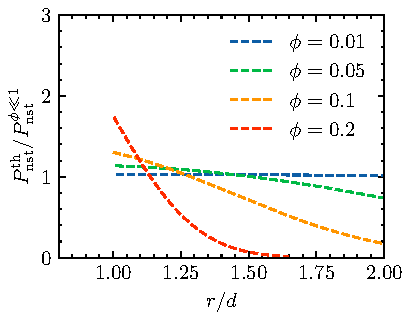
\includegraphics[height=0.3\textwidth]{image/HOMOGENEOUS_final/Dist/Theory.pdf}
    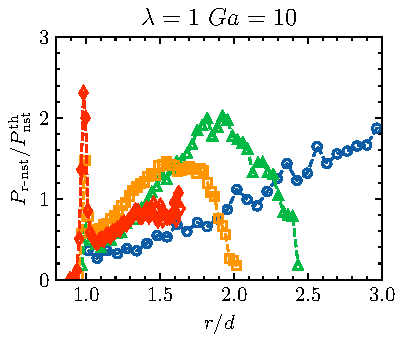
\includegraphics[height=0.3\textwidth]{image/HOMOGENEOUS_final/Dist/Pr_l_1_Ga_10.pdf}
    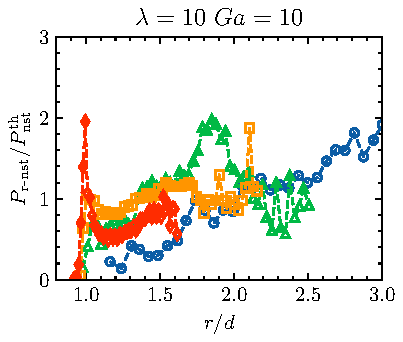
\includegraphics[height=0.3\textwidth]{image/HOMOGENEOUS_final/Dist/Pr_l_10_Ga_10.pdf}
    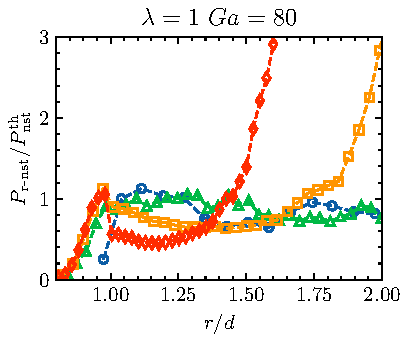
\includegraphics[height=0.3\textwidth]{image/HOMOGENEOUS_final/Dist/Pr_l_1_Ga_80.pdf}
    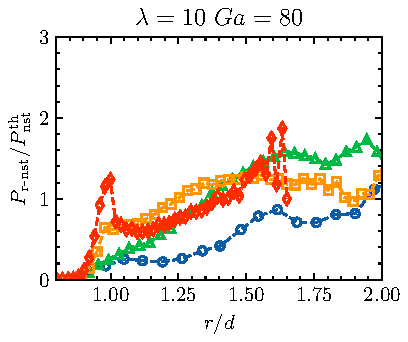
\includegraphics[height=0.3\textwidth]{image/HOMOGENEOUS_final/Dist/Pr_l_10_Ga_80.pdf}
    \caption{
    Ratio of the radial probability density functions, $P_\text{r-nst}/P_\text{nst}^\text{th}$ with $P_\text{nst}^\text{th}$ given by \ref{eq:Pnst_dilute}, as functions of the dimensionless distance $r/d$, for $Ga = 80$, $Ga =10$, $\lambda = 1$ and $\lambda = 10$.
    % (dashed lines) Theoretical prediction : $P_\text{nst}^{th}/P_\text{nst}^{\phi \ll 1}$. 
    (symbols) DNS results of $P_\text{r-nst}(r) / P_\text{nst}^{\phi \ll 1}$ with :
    ($\pmb\bigcirc$) $\phi = 0.01$; ($\pmb\triangle$) $ \phi = 0.05$; ($\pmb\square$) $\phi = 0.1$ ($\pmb\lozenge$) $\phi = 0.2$.
    For $r<d$ we arbitrarily set $P_\text{nst}^\text{th} = 1$ so that $P_\text{r-nst}$ can be visualized. 
    This, is why the ratio  $P_\text{r-nst}/P_\text{nst}^\text{th}$ may exhibit discontinuity at $r/d =1$. 
    }
    \label{fig:Pr}
\end{figure}
We plotted in \ref{fig:Pr} the ratio $P_\text{r-nst}/P_\text{nst}^\text{th}$ as functions of the dimensionless distance $r/d$.
This is particularly interesting to study since it represents the effect of fluid dynamics and particle interactions on the nearest pair distribution, given that $P_\text{nst}^\text{th}$ already accounts for the geometric effects due to finite volume fraction $\phi$. 
In \ref{fig:Pr} we display the distributions for two different viscosity ratios and multiple volume fractions. 
Let us first examine the low inertia cases displayed in \ref{fig:Pr} (top). 
It is seen that at $\phi = 0.01$ we have $P_\text{r-nst} < P_\text{nst}^\text{th}$ for roughly $r/d < 2$.
This indicates that the likelihood of finding the nearest neighbor in the vicinity of the \textit{test particle} (i.e. $r/d<2$) is less than $P_\text{nst}^\text{th}$.
In opposition, at $r/d>2$ the probability density $P_\text{r-nst}$ is higher than $P_\text{nst}^\text{th}$.
In these cases, i.e. $\phi = 0.01$ and $\lambda = 10, 1$, the maximum of $P_\text{r-nst}/P_\text{nst}^\text{th}$ is reached at $r/d \approx 3$, indicating that on average, more pairs of nearest neighbors are found with a significant distance between each other compared to the random cases. 
For comparison, the distance to the nearest neighbor in an ordered array of particles in a cubic lattice is  $\frac{1}{2}\left[4\pi/(\phi 3)\right]^{1/3} \approx 3.74$ at $\phi = 0.01$.
Additionally, it is interesting to notice that $P_\text{r-nst}/P_\text{nst}^\text{th}(r/d =1) \approx 0$ while $P_\text{nst}^\text{th}(r/d =1) = 1$ (see \ref{fig:torquato}), implying that in this regime, very few particle-particle contacts are observed. 
Overall, hydrodynamic interactions appear to maintain particles at a relatively greater distance from each other compared to the random case in the low inertia and dilute regime.
As $\phi$ increases, the maximum of $P_\text{r-nst}/P_\text{nst}^\text{th}$ is found at lower values of $r/d$. 
At $\phi = 0.2$ a local maximum is observed at $r/d = 1$ and another at $r/d = 1.5$.
This signifies that the probability of finding a nearest neighbor between the spherical shells of radius $r/d = 1$ and $r/d = 1.5$ is lower than the theoretical prediction.
In contrast, the density of finding a particle outside this area seems greater than $P_\text{nst}^\text{th}$. 
Therefore, at large $\phi$, hydrodynamic interactions seem to induce fewer neighbors at mid-distance ($1<r/d<1.5$) from \textit{test particle} than the theoretical prediction. 
At this stage, no significant differences between the cases $\lambda = 1$ and $\lambda = 10$ have been identified.

Let us now focus on the inertial cases displayed on \ref{fig:Pr} (bottom). 
For $\phi = 0.01, 0.05$ and $\lambda=1$, we observe that $P_\text{r-nst}$ is in reasonable agreement with $P_\text{nst}^\text{th}$.  
For higher volume fractions at the same $\lambda$, we observe that $P_\text{r-nst}/P_\text{nst}^\text{th} < 1$ at moderate values of $r/d$,  indicating that hydrodynamic interactions seem to repel particles from each other. 
Then, for increasing values of $r/d$, $P_\text{r-nst}/P_\text{nst}^\text{th}$ reaches surprisingly high values.  
This can be explained by the following observation. 
As demonstrated in \ref{fig:images} and \ref{fig:Pnst_high_Ga} the microstructure is highly inhomogeneous in these cases ($Ga =80$ and $\lambda =1$), specifically they exhibit clusters of particles and layered structures.
Additionally, note that the presence of clusters ultimately implies the presence of particle-free regions as $\phi$ must remain constant. 
Consequently, the likelihood for a particle to be far from its nearest neighbors is increased, as particle-free regions allow some particles to be isolated from all others by being located at the center of these regions.
Thus, this explains the high value of $P_\text{nst}^\text{th}$ at large $r/d$ in \ref{fig:Pr} (bottom-left) compared to the random distribution $P_\text{nst}^\text{th}$ which is nearly null at these values of $r/d$ (see \ref{fig:torquato}). 
In contrast, for  $\lambda = 10$ and $\phi=0.01,0.05$, it becomes evident that fewer particles are observed in close vicinity to the \textit{test particle} compared to $P_\text{nst}^\text{th}$. 
Consequently, for $Ga = 80$ and $\phi \le 0.05$, hydrodynamic interactions seem to be more significant for $\lambda=10$ than $\lambda=1$, as we observe lower values of $P_\text{r-nst}/P_\text{nst}^\text{th}$ in the close vicinity of the \textit{test particle} in the former case.
Additionally, for higher volume fraction still at $\lambda = 10$, the behavior described above where we identified very high values of $P_\text{r-nst}/P_\text{nst}^\text{th}$ at large $r/d$, cannot be observed here.
This might be because the suspension is more evenly dispersed in these cases.  
Lastly, it is clear from \ref{fig:Pr} that the particles deform at contact, as witnessed by the non-vanishing value of $P_\text{r-nst}$ for $r/d<1$.
This phenomenon is particularly pronounced for the case $Ga = 80$ and $\lambda =1$. 
This is consistent with the high values of droplet aspect ratios reported in \ref{ap:deformation} \ref{fig:chi} for this case.



To conclude these observations, we note that both the radial and azimuthal distributions were affected by the inertial effects measured by the \textit{Galileo} number. 
The major effect of high inertia is the generation of strong anisotropy in the particle pair distribution and a more important concentration of neighboring particles at $r/d < 1$. 
Furthermore, the density at contact and close contact of the \textit{test particle} is higher for increasing volume fractions as predicted by $P_\text{nst}^\text{th}$  (see \ref{fig:torquato}).
This tendency persists even though it is influenced by the particles' hydrodynamic interactions, as evidenced by \ref{fig:Pr}. 
Overall, $P_\text{nst}^\text{th}$ seems to represent $P_\text{r-nst}$ well only in the cases where $\lambda =1$, $Ga = 80$ and $\phi \le 0.05$. 
It must be concluded that, in this regime, fluid dynamics and particle interactions have the least influence on the final pair distribution, in contrast to the low inertia or viscous droplet regime ($\lambda =10$).
% as depicted by \ref{fig:torquato} and vekcrified in \ref{fig:Pr}. 
Thus, the viscosity ratio strongly impacts the microstructure, but only at high $Ga$, whereas at low $Ga$, the change in viscosity ratio has no notable impact on $P_\text{nst}$. 
% Lastly, note that \ref{eq:torquato} provides a significantly improved prediction of the radial distribution compared to $P_\text{nst}^{\phi \ll 1}$ \eqref{eq:Pnst_dilute} (see \ref{fig:Pr}). 
% Indeed, the DNS results show that $P_\text{r-nst}$ follows trends similar to $P_\text{nst}^\text{th}$ as $\phi$ increases. 
% Quantitative agreements are particularly observed for high inertia cases.

\subsection{Macroscopic modeling of the microstructure}
%Up to now we have presented visualizations of the microstructure with 2D or 1D distributions. 
%For a more concise description we would like to adopt a different approach. 
%Following \citet{zhang2023evolution} we opt to describe the microstructure using the second moment of $P_\text{nst}$ with respect to \textbf{r}, which reads
Until now, we have depicted the microstructure through 2D or 1D distributions. To provide a more succinct description, we propose a different method. 
Inspired by \citet{zhang2023evolution}, we will characterize the microstructure using the second moment of $P_\text{nst}$ with respect to $\mathbf{r}$, which is expressed as
\begin{equation}
    \textbf{R} =\frac{1}{n_p} 
    % \int_0^\infty 
    \int_{\mathbb{R}^3} 
    \textbf{rr} P_\text{nst}(\textbf{r}) d\textbf{r}.
    \label{eq:R}
\end{equation}
The tensor $\textbf{R}$ allows us to measure the mean-square distance between a particle and its nearest neighbor in the three dimensions of space.
%This second-rank tensor measures the spread of the nearest neighbor distribution in a given direction. 
It is worth noting that such a quantity is computable only because $\lim_{|\textbf{r}|\to \infty} P_\text{nst}(\textbf{r}) = 0$, which enables the integral of \ref{eq:R} to converge. 
This would not be the case for classical pair distributions, which is one of the main reasons for using the \textit{nearest particle statistics} framework. Since our objective is to measure the anisotropy of the microstructure, we are particularly interested in the deviatoric part of this tensor, namely
\begin{equation*}
    \textbf{A} = \textbf{R} - \frac{1}{3}  \text{tr}(\textbf{R}) \bm\delta.
\end{equation*}
Where $\bm\delta$ is the unit tensor and 
$\textbf{A}$ represents the likelihood of having a particle in a given direction compared to the mean radial square distance. 
Therefore, in an isotropic suspension, we have $A_{xx} = A_{yy} = 0$, where $y$ represents the coordinate aligned with gravity. 
In a situation like the one depicted in \ref{fig:images} (left), particles are more likely to have closer neighbors on the lateral sides rather than vertically positioned, hence  $A_{yy} < 0$ and $0 < A_{xx}$. 


To facilitate the understanding of the subsequent findings, it is helpful to calculate the distance $r_m$. 
This distance represents the average distance to the closest neighboring particle within a random arrangement of dilute hard spheres. 
Through direct integration of \ref{eq:Pnst_dilute}, we get
\begin{align}
    \frac{r_m^2}{d^2}
    = 
    % \frac{1}{n_p}
    \frac{1}{d^2}
    \int_{\mathbb{R}^3} r^2 P_\text{nst}^{\phi \ll 1}(\textbf{r}) d\textbf{r} 
    =  \frac{\Gamma\left({{5}\over{3}} , 8\,\phi\right)}{8^{2/3}}\frac{e^{8\phi}}{\phi^{2/3}},
    % = d^2{{4^{{{2}\over{3}}}\,\Gamma\left({{5}\over{3}} , 8\,\phi\right)
    % \,e^{8\,\phi}}\over{2^{{{10}\over{3}}}\,\phi^{{{2}\over{3}}}}}
\end{align}
where $\Gamma(z,a) = \int_a^\infty t^{z-1} e^{-t} dt$ is the upper incomplete gamma function.
\begin{figure}
  \centering
  \includegraphics[height = 0.3\textwidth]{image/HOMOGENEOUS_final/PA/rm.pdf}
  \caption{Dimensionless radial distance $r_m/d$ to the nearest neighbor for a random distribution.}
  \label{fig:agee}
\end{figure}
Since the upper incomplete gamma function is relatively uncommon, we have illustrated the dimensionless distance $r_m/d$ as a function of $\phi$ in \ref{fig:agee} to aid understanding. This figure clearly shows that $r_m$ decreases as $\phi$ increases.
%Since the upper incomplete gamma function is not so common we have plotted in \ref{fig:ap:agee} the dimensionless distance $r_m/d$ in terms of $\phi$ to help comprehension. As can be seen from this figure $r_m$ is a decreasing function of $\phi$.

\begin{figure}[h!]
    \centering
    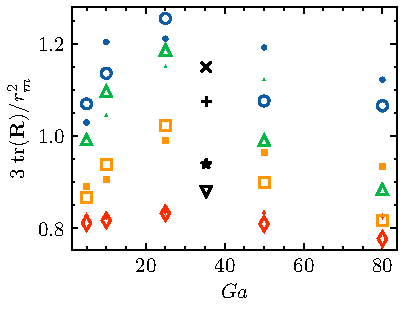
\includegraphics[height=0.3\textwidth]{image/HOMOGENEOUS_final/PA/trR.pdf}
    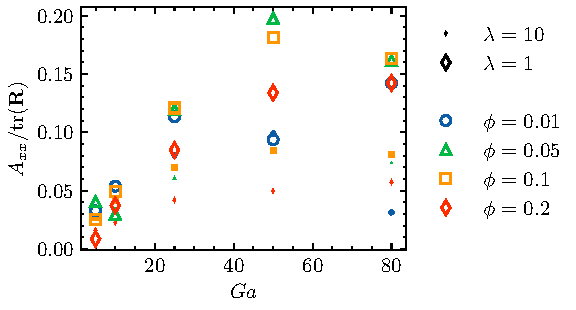
\includegraphics[height=0.3\textwidth]{image/HOMOGENEOUS_final/PA/Axx.pdf}
    \caption{
        (left) Dimensionless trace of $\textbf{R}$ as a function of the volume fraction.%Trace of the second moment of the probability density function $P_\text{nst}(\textbf{r})$ divided by the square diameter of the particles $d^2$. 
        (right) Horizontal components of the anisotropy tensor divided by the trace of $\textbf{R}$. %the second moment of the probability density function.
    ($\pmb\bigcirc$) $\phi = 0.01$; ($\pmb\triangle$) $ \phi = 0.05$; ($\pmb\square$) $\phi = 0.1$ ($\pmb\lozenge$) $\phi = 0.2$.
    The hollow symbols correspond to $\lambda = 1$, the filled symbols to $\lambda = 10$.
    % For $r<d$, we arbitrarily set $P_\text{nst}^\text{th} = 1$ so that the distribution can be visualized.
    Black symbols represent the results of \citet{zhang2023evolution} for sedimenting spherical particles with $\phi = 0.016,0.056,0.134,0.262$ and $\zeta = 2.56$. %$\phi = 0.0168,0.0565,0.1341,0.2622$ 
    Corresponding to $\pmb\times,\pmb +, \pmb\star , \pmb\triangledown$, respectively.
    }
    \label{fig:A}
\end{figure}
In \ref{fig:A} (left), the dimensionless mean square distance between nearest neighbors, represented as $3\cdot\text{tr}(\textbf{R})/r_m^2 = \textbf{R}:\bm\delta/r_m^2$, is illustrated for all configurations explored in this study. 
The simulation marked by the symbol \textcolor{col1}{$\pmb\circ$} in \ref{fig:A} (left), corresponding to parameters $\lambda = 1$, $Ga = 80$, and $\phi = 0.01$, yields a value of $\bm\delta:\textbf{R}/r_m^2 \approx 1$. 
This observation agrees with the quasi-hard-sphere distribution previously reported in this case in \ref{fig:Pr} (left).
The dependence of the mean square distance on the volume fraction is also displayed on \ref{fig:A} (left). 
We observe a decrease in $\bm\delta:\textbf{R}/r_m^2$ as $\phi$ increases, indicating that particles tend to come closer to each other on average compared to a dilute random distribution of hard spheres. 
This observation, as highlighted by \citet{zhang2023evolution}, suggests the emergence of clusters when increasing the particle volume fraction. 
Note that this trends is not due to hydrodynamic effect but rather to geometrical effect already predicted by $P_\text{nst}^\text{th}$ (see \ref{fig:torquato}). 
The dependence on the \textit{Galileo} number is non-monotonic. 
Indeed $\bm\delta:\textbf{R}/r_m^2$ increases until $Ga = 25$ and then decreases until $Ga = 80$. We also note that the distance to the nearest neighbor is not significantly affected by the viscosity ratio, particularly when dealing with high-volume fractions. 
In \ref{fig:A} (left), the symbols $\pmb\star$, $\pmb\times$, $\pmb +$, and $\pmb\triangledown$ depict the findings from the study conducted by \citet{zhang2023evolution} on the sedimentation of solid spheres in a liquid.
As observed, the value of $\textbf{R}:\bm\delta$ is, on average, closer to the mean $r_m^2$ than our simulations, but it maintains the same trend, i.e., clusters appear as the volume fraction increases.
 
\ref{fig:A} (right) illustrates the anisotropy of the microstructure. We can see on \ref{fig:A} (right) that we have $A_{xx} \ge 0$ for nearly all our cases, meaning that the emulsion is either isotropic ($A_{xx} = 0$), or exhibits a tendency towards a horizontal alignment of particles on average ($A_{xx} >0$). % or with particles that are in average more aligned horizontally ($A_{xx} >0$). 
%Moreover $A_{xx}$ increases with $Ga$ until $Ga = 50$ where we reach a maximum, and then decrease until $Ga =80$  but still remains consequent. 
Additionally, $A_{xx}$ rises with $Ga$ up to $Ga = 50$, reaching a peak, and subsequently decreases until $Ga = 80$, although it remains significant.
In agreement with the remarks of the previous section, the value of $A_{xx}$ is greater for $\lambda = 1$ and lower for  $\lambda = 10$.
Although not obvious at first, we observe a non-monotonic trend with the volume fraction. $A_{xx}$ increases up to a peak value at $\phi = 0.1$ (indicated by \textcolor{col3}{$\pmb\square$} on \ref{fig:A} (right)), but then decreases for $\phi=0.2$ (shown by the \textcolor{col4}{$\pmb\lozenge$} symbols). %$A_{xx}$ first increases up to a maximum value for $\phi =0.1$ (represented by \textcolor{col3}{$\pmb\square$} on \ref{fig:A} (right)) and then decreases for $\phi=0.2$ (represented by the \textcolor{col4}{$\pmb\lozenge$} symbols).
%Although, it is not quite obvious we observe a non-monotonic trend with the volume fraction, $A_{xx}$ first increases up to a maximum value for $\phi =0.1$ (represented by \textcolor{col3}{$\pmb\square$} on \ref{fig:A} (right)) and then decreases for $\phi=0.2$ (represented by the \textcolor{col4}{$\pmb\lozenge$} symbols). 
This implies that at a certain volume fraction, around $\phi \approx 0.1$, higher $\phi$ makes the microstructure more isotropic, while at low volume fraction ($\phi < 0.1$), increasing $\phi$ favors the side-by-side configuration.
This phenomenon of isotropization at high $\phi$ has been reported in other studies such as in \citet{seyed2021sedimentation} for sedimentation of solid particles. 
However, at high \textit{Galileo} numbers, it seems that this effect is less pronounced. 


To conclude, we classify the microstructure into four classes :
(1) The homogeneous microstructure.
(2) The non-homogeneous but isotropic microstructure with $\textbf{R}:\bm\delta > r_m^2$, or dispersed arrangement. %ordered array.
(2 bis) The non-homogeneous but isotropic microstructure with $\textbf{R}:\bm\delta < r_m^2$, or clustering. 
(3) The non-homogeneous and non-isotropic microstructure or layering ($\textbf{A}\neq \textbf{0}$). 
Each of these types is characterized by specific values of $\textbf{R}$; they are reported in \ref{tab:microstructure}. 

\begin{table}[h!]
    \caption{Microstructure classification}
    \label{tab:microstructure}
    \centering
    \begin{tabular}{|lccccc|} \hline
        Microstructure types & Homogeneous & Isotropic & \ref{fig:scheme_clusters} & $\textbf{R}:\bm\delta/r_m^2$ & $A_{xx}/tr(\textbf{R})$ \\
        Homogeneous & Yes & Yes &(\textit{Case 1}) & $ \approx 1$ & $\approx 0$ \\
        Dispersed &  No & Yes  &(\textit{Case 2}) & $ > 1$ & $\approx 0$ \\
        Clustering &  No & Yes  &(\textit{Case 2}) & $ < 1$ & $\approx 0$ \\
        Layering &    No & No  &(\textit{Case 4}) & $ - $ & $< 1$\\ \hline
    \end{tabular}
\end{table}
Additionally, to highlight the dependence of $\textbf{R}$ on $\phi$ and $Ga$, we display the values of $A_{xx}/tr(\textbf{R})$ and $\textbf{R}:\bm\delta/r_m^2$ in phase diagrams on \ref{fig:phase}.
We observe that the mean square particle distance compared to a random case decreases when increasing the volume fraction and is globally higher for viscous particles ($\lambda = 10$).
Meanwhile, the likelihood of finding the nearest neighboring particle on the horizontal is greater for $\lambda=1$ than $\lambda = 10$, and it is globally increasing with  $Ga$ and non-monotonic with $\phi$. 
We reach the configuration with the maximum anisotropy for both viscosity ratios at $Ga \approx 50$ and $\phi \approx 0.1$. 
%We conclude that 

\begin{figure}[h!]
    \centering
    \begin{tikzpicture}[scale=0.8]
        \node (img) at (0,0) {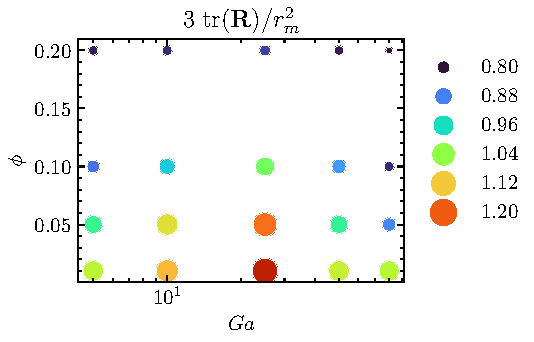
\includegraphics[height=5.5cm]{image/HOMOGENEOUS_final/PA/phase_Rtr_l_1.pdf}};
        % \draw[dashed] (10cm,-1.6) ellipse (3 and 2);
        \node (txt) at (-2,1) {Clustering};
        \node (txt) at (-1,-1.6) {Dispersed};
        \draw[dashed] ($(-1,-1.6) + (-10:3 and 2)$(P) arc
        (-10:155:3 and 2);
        \node (img) at (10.5,0) {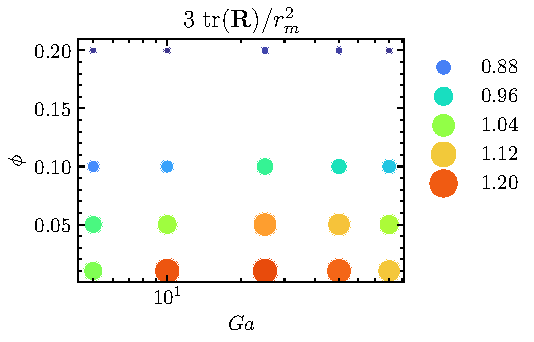
\includegraphics[height=5.5cm]{image/HOMOGENEOUS_final/PA/phase_Rtr_l_10.pdf}};
        % \draw[dashed] (10cm,-1.6) ellipse (3 and 2);
        \node (txt) at (8.5,1) {Clustering};
        \node (txt) at (10,-1.6) {Dispersed};
        \draw[dashed] ($(10,-2) + (-10:3 and 2)$(P) arc
        (-10:180:3 and 2);
    \end{tikzpicture}
    \begin{tikzpicture}[scale=0.8]
        \node (img) at (0,0) {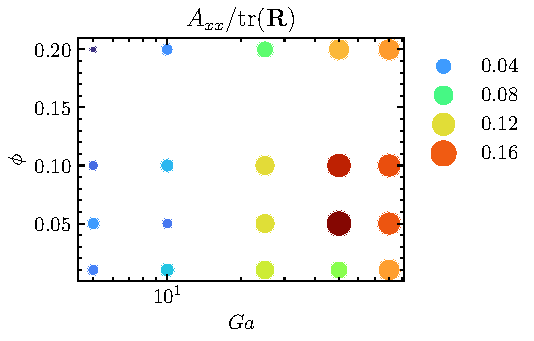
\includegraphics[height=5.5cm]{image/HOMOGENEOUS_final/PA/phase_axx_l_1.pdf}};
        \draw[dashed] (1.4,0.3) ellipse (1.5 and 2.5);
        \node (txt) at (1.4,1) {Anisotropic};
        \node (txt) at (-2,1) {Isotropic};

        \node (img) at (10.5,0) {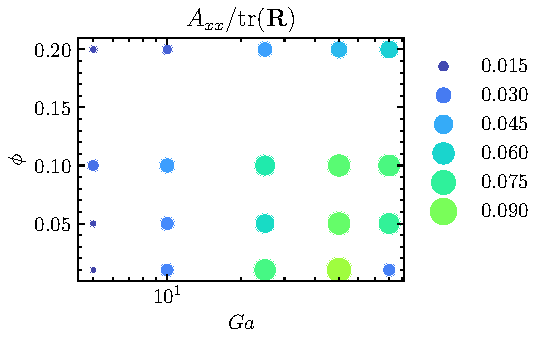
\includegraphics[height=5.5cm]{image/HOMOGENEOUS_final/PA/phase_axx_l_10.pdf}};
        % \draw[dashed] (11.7,-0.5) ellipse (0.75 and 1.75);
        % \node (txt) at (11.7,1) {Anisotropic};
        \node (txt) at (8,1) {Isotropic};
    \end{tikzpicture}
    \caption{
        (top) Phase diagram of the dimensionless mean square distance to the nearest neighbor, $\bm\delta:\textbf{R}/r_m^2$.
        (bottom) Phase diagram of the dimensionless horizontal components of the anisotropy tensor, $A_{xx}/\text{tr}(\textbf{R})$.  
        (left) Iso-viscous emulsion $\lambda = 1$.
        (right) Viscous droplets $\lambda = 10$ }
    \label{fig:phase}
\end{figure}

\subsubsection*{Discussion}
%Although, previous studies mainly focused on bubbles or solid particles, it is reasonable to compare the $\lambda = 1$ and $\lambda = 10$ simulations, to the former and the latter cases, respectively. 
%In \citet{bunner2002dynamics} they performed tri-periodic simulation of buoyant bubbles at $Re \approx 10-30$ for various $\phi$.
%They reported a preference for the bubbles to be aligned in pair.
While earlier studies primarily focused on bubbles or solid particles, it is reasonable to draw parallels between simulations with $\lambda = 1$ and $\lambda = 10$, corresponding to the former and latter scenarios, respectively. In \citet{bunner2002dynamics}, buoyant bubbles were simulated in a tri-periodic setup at Reynolds numbers around 10-30 for various volume fractions ($\phi$). The authors noted a tendency for the bubbles to align in horizontal pairs. % a finding that aligns with our observations.
This observation is consistent with what we observe in \ref{fig:phase} ($\lambda = 1$) since the anisotropy tensor is relatively high ($A_{xx} \approx 0.15$) for $Ga = 25$ (which corresponds roughly to $Re = 25$). 
% Additionally, it is seen that these layers structures are lost at lower volume fraction ($\phi = 0.01$). 
Moreover, \citet{zhang2021direct} conducted Direct Numerical Simulations (DNS) of buoyant bubbly flows within tri-periodic domains. The Reynolds numbers varied from $Re=18$ to $22.8$ across different volume fractions, $\phi$, ranging from $0.05$ to $0.2$, with a fixed Galileo number, $Ga$, of $29$. They observed the presence of anisotropic clusters for $\phi > 0.1$, while noting their absence at lower volume fractions. This observation aligns with findings depicted in \ref{fig:phase} (left), where a small decrease in the value of $A_{xx}$ may be observed for the lowest $\phi$.
%Furthermore, in \citet{zhang2021direct} they carried out DNS of buoyant bubbly flows in tri-periodic domains.
%Their \textit{Reynolds} numbers range form $Re=22.5\to 18$ for various volume fraction : $\phi = 0.05\to 0.2$ and a fixed \textit{Galileo} number of $Ga = 29$. 
%They observe anisotropic clusters for $\phi >0.1$ as well, and they report that at lower volume fraction these structures are not present. 
%It is consistent with the results reported in \ref{fig:phase} (left) where we can see that the value of $A_{xx}$ clearly decreases for lower $\phi$. 

For solid particles at $Ga = 144$, it is observed in \citet{shajahan2023inertial} that vertical rafts of particles are formed in the dilute regime ($\phi \approx 0.02$). This phenomenon was attributed to a well-defined wake around individual particles, which effectively traps neighboring particles within the wake without causing repulsion toward the sides. %This effect was explained by the presence of a more developed wake for dilute solid particles which trap neighboring particles within the wake without repulsing it on the sides. 
In our case, we notice a greater concentration of particles in the vertical directions for $\lambda = 10$ compared to $\lambda = 1$ at $Ga = 80$, as evidenced by the smaller value of $A_{xx}$ in the former case. Although not immediately apparent, this phenomenon could be attributed to similar factors, namely, the wake of the viscous drop potentially inducing fewer instances of particles aligning side-by-side and more instances of vertically stable configurations. DNS at higher $Ga$ and $\lambda$ would be necessary to confirm or not the presence of the wake trapping effect. %To conclusively confirm or refute the presence of this wake-trapping effect, it would be necessary to conduct DNS at higher $Ga$ and $\lambda$ values.
%In our case we observe more particles in the verticals directions for $\lambda = 10$ than $\lambda =1$ at $Ga =80$, since $A_{xx}$ is smaller in the former cases.
%Although it is not quite obvious it might be the consequence of the same effects, i.e., the wake of the viscous drop might induce less side-by-side configuration and more vertical nearly stable configuration. 
%DNS at higher $Ga$ and $\lambda$ would be necessary to confirm or not the presence of the wake trapping effect.
%In our case we could not observe such a phenomenon, meaning that it might arise at larger \textit{Galileo} number or that the approximation of solid particle at for $\lambda = 10$ is too coarse.
In the moderately dense regime,  $0.02 < \phi \le 0.1$  \citet{shajahan2023inertial} identified more configurations of particles situated side-by-side. 
As mentioned above, even if it is less pronounced than for $\lambda = 1$, we indeed observe that $A_{xx}$ is higher in these cases; see \ref{fig:phase} (right). 
Additionally, \citet{almeras2021statistics} carried out experiments of liquid-solid fluidized bed with spherical particles. 
Their Reynolds numbers range between $150\leq Re \leq 360$ depending on the volume fraction $0.14 \leq \phi \leq 0.42$.
It is observed that particles are most concentrated on the horizontal plane of the reference particle when $\phi = 0.14$.
If the $\lambda = 10$ cases follow the same trend, it is reasonable to expect that the probability of horizontal configurations, already predominant at $Ga =80$, will continue to increase for higher \textit{Galileo} at $\phi  \approx 0.1$.

We would like to end this comparison with the literature with the study of \citet{yin2008lattice} which compares the microstructure of suspensions of rising bubbles with suspensions of sedimenting solid particles.
%They studied two \textit{Reynolds} numbers and two volume fractions : $Re = 5,20$ and  $\phi = 0.05, 0.2$, respectively.
%It is found that :
The study encompasses two Reynolds numbers ($Re = 5, 20$) and two volume fractions ($\phi = 0.05, 0.2$). Their findings reveal that: 
\enquote{    
     microstructure in bubble
    suspensions is more anisotropic and inhomogeneous than
    solid particle suspensions of the same volume fraction and
    \textit{Reynolds} number.    
}. 
%Although we compare emulsions with varying droplets' viscosity rather than bubbles and solid particles' suspension, our conclusion regarding the anisotropy of the flow is consistent with their study.
%Additionally, it is also observed in \citet{yin2008lattice} that the microstructure shape has a clear impact on the mean rising velocity of the dispersed phase.
%Indeed, they observed that a power-law function of $(1-\phi)$ fit perfectly the rising velocity of random and isotropic suspensions, while it is not the case when the microstructure exhibit anisotropic structures. 
%Therefore, as stated in introduction, the knowledge of the microstructure shape (reported in \ref{fig:phase}), is of utmost importance in the objective of building realistic averaged models. 
While our analysis focuses on emulsions with varying droplet viscosities rather than bubbles and suspended solid particles, our findings regarding the flow anisotropy align with the study of \citet{yin2008lattice}. 



% In the following we try to explain the origin of the striking difference between $\lambda = 1$ and $\lambda = 10$ on the particle pair distribution.
% With this objective in mind, we present a meticulous analysis of the particle time of interaction as well as the particles relative averaged velocity fields. 


\section{Conclusion}
\label{sec:conclusion}
\section{Conclusion}

% \citet{einstein1905neue,taylor1932viscosity} demonstrated how the first moment of the hydrodynamic forces (Stresslet) applied on a particle immersed in pure linear flow induced an additional viscosity to the mixture. 
% Later~\citet{zhang1994ensemble,lhuillier1996contribution,jackson1997locally,zhang1997momentum} demonstrated that the second moment of forces were also contributing to the stresses inducing a non-newtonian behaviors, even in the Stokes and dilute limit.  

In this work we computed the moments of force on the surface of a test droplet in the situation of uniform relative motions between the droplet and the continuous phase. 
We considered low but finite Reynolds number $Re$. 
The averaged first moment of force is given by~\ref{eq:forces_reformulated2_avg}, scales as $O(\rho_f \phi u_r^2)$, hence contributing to the averaged Stress of the suspension on the same ground as  \citet{einstein1905neue} or \citep{taylor1932viscosity} correction to the viscosity of the mixture. 
In a lesser extend the inertial part of the second moment also contribute to the Rheology. 
This first point constitutes the main result of the paper. 

Others important conclusion reached through this work includes: a general reciprocal formula to derive the forces and moments on droplets, and the explicit appearing of the velocity variance term in the drag force term. 







\appendix



\section{Additional information}
\label{ap:age} 

\begin{figure}[h!]
  \centering
  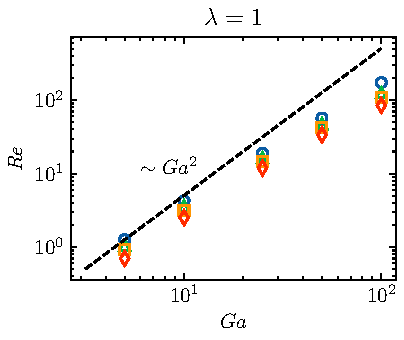
\includegraphics[height = 0.3\textwidth]{image/HOMOGENEOUS_NEW/CA/Re_l_1.pdf}
  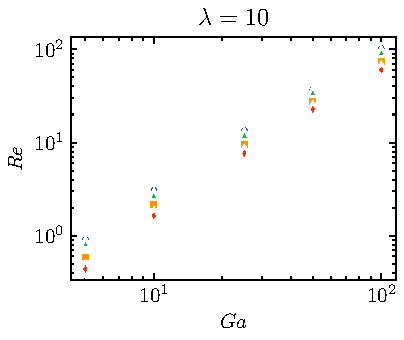
\includegraphics[height = 0.3\textwidth]{image/HOMOGENEOUS_NEW/CA/Re_l_10.pdf}
  \caption{
      Averaged Reynolds number based on the averaged drift velocity, $Re = \rho_fU d /\mu_f$, with $U = |\textbf{u}_p - \textbf{u}_f|$.
      $\textbf{u}_p$ and $\textbf{u}_f$ are the particle and fluid phase volume and time averaged velocity.
  }
  \label{fig:Reall}
\end{figure}

\begin{table}  
\begin{tabular}{c|c|c|c|l}
  calls  &  total  &   self  & \% total  & function \\ \hline
  10636901 &  4861.39 &  4861.39  &   31.8\% (28.4\% - 36.7\%) &   mpi\_boundary\_level():grid/multigrid-mpi.h:83\\
     53604 &  3097.64 &  1988.97  &   13.0\% (10.8\% - 14.7\%) &   project():poisson.h:501\\
     26802 &  2022.99 &  1236.57  &    8.1\% ( 7.3\% -  8.8\%) &   viscosity():viscosity.h:173\\
    107208 &  1984.59 &  1223.33  &    8.0\% ( 6.9\% -  8.9\%) &   heights():heights.h:281\\
     26802 &  2499.81 &  1099.66  &    7.2\% ( 6.1\% -  7.9\%) &   vof\_0():vof.h:365\\
   3155070 &  983.66  & 983.66    &  6.4\% ( 3.9\% -  9.1\%)   & mpi\_all\_reduce0():common.h:683\\
     26802 &  2372.23 &  896.09   &   5.9\% ( 5.1\% -  6.5\%)  &  advection\_term():navier-stokes/centered.h:323\\
     26802 &  1583.59 &  645.89   &   4.2\% ( 4.1\% -  4.3\%)  &  no\_coalescence():./no-coalescence.h:419\\
      2681 &  584.39  & 372.15    &  2.4\% ( 2.4\% -  2.5\%)   & track\_bub():RS.c:124\\
    321624 &  546.74  & 340.36    &  2.2\% ( 1.8\% -  2.6\%)   & reconstruction():fractions.h:476\\
    107208 &  2777.30 &  303.23   &   2.0\% ( 1.6\% -  2.4\%)  &  curvature():curvature.h:621\\
     69275 &  992.44  & 254.14    &  1.7\% ( 1.4\% -  1.8\%)   & tag():tag.h:268\\
     26802 &  328.67  & 202.85    &  1.3\% ( 1.1\% -  1.5\%)   & acceleration\_0():iforce.h:133\\
     26802 &  2257.27 &  178.19   &   1.2\% ( 0.8\% -  1.3\%)  &  projection():navier-stokes/centered.h:430\\
     26802 &  2142.30 &  119.30   &   0.8\% ( 0.5\% -  0.9\%)  &  viscous\_term():navier-stokes/centered.h:362\\
     26802 &  145.95  & 116.09    &  0.8\% ( 0.5\% -  0.9\%)   & acceleration\_2():RS.c:166\\
     26803 &  111.60  & 111.57    &  0.7\% ( 0.5\% -  0.8\%)   & properties\_0():two-phase-generic.h:101\\
     26802 &  172.09  & 100.18    &  0.7\% ( 0.5\% -  0.8\%)   & acceleration():navier-stokes/centered.h:386\\
     69275 &   68.91  &  68.88    &  0.5\% ( 0.4\% -  0.5\%)   & z\_indexing():grid/multigrid-mpi.h:145\\
       118 &   59.59  &  59.59    &  0.4\% ( 0.2\% -  0.8\%)   & compose\_image():view.h:409\\
     26802 &   64.69  &  34.48    &  0.2\% ( 0.2\% -  0.3\%)   & tracer\_advection\_1():./no-coalescence.h:446\\
        59 &  129.57  &  28.81    &  0.2\% ( 0.1\% -  0.2\%)   & movies():RS.c:244\\
     26803 &   92.48  &  27.24    &  0.2\% ( 0.1\% -  0.2\%)   & stability\_1():tension.h:64\\
     26803 &   24.42  &  21.33    &  0.1\% ( 0.1\% -  0.1\%)   & stability():navier-stokes/centered.h:226\\
  43894361 &  3001.24 &    5.50   &   0.0\% ( 0.0\% -  0.0\%)  &  boundary\_internal():grid/cartesian-common.h:450\\
  42061052 &   25.50  &   3.61    &  0.0\% ( 0.0\% -  0.0\%)   & interpolate():grid/cartesian-common.h:815\\
       472 &    2.31  &   2.31    &  0.0\% ( 0.0\% -  0.0\%)   & draw\_vof():draw.h:1052\\
     58554 &   25.92  &   0.87    &  0.0\% ( 0.0\% -  0.0\%)   & reduce\_bubbles():./no-coalescence.h:158\\
         1 &  15287.89&     0.73  &    0.0\% ( 0.0\% -  0.0\%) &   run():run.h:37\\
         1 &    0.28  &   0.28    &  0.0\% ( 0.0\% -  0.0\%)   & init\_0():RS.c:149\\
     26802 &  2777.57 &    0.27   &   0.0\% ( 0.0\% -  0.0\%)  &  acceleration\_1():tension.h:94\\
       236 &   38.81  &   0.21    &  0.0\% ( 0.0\% -  0.0\%)   & squares():draw.h:1375\\
    %    118 &   59.64  &   0.05    &  0.0\% ( 0.0\% -  0.1\%)   & save():view.h:529\\
    %  63404 &    0.06  &   0.03    &  0.0\% ( 0.0\% -  0.0\%)   & interpolate():grid/cartesian-common.h:816\\
    %      1 &    0.02  &   0.02    &  0.0\% ( 0.0\% -  0.0\%)   & defaults\_3():iforce.h:38\\
    %      1 &    0.01  &   0.01    &  0.0\% ( 0.0\% -  0.0\%)   & defaults\_2():two-phase-generic.h:26\\
    %  26802 &  1583.60 &    0.01   &   0.0\% ( 0.0\% -  0.0\%)  &  vof\_1():./no-coalescence.h:430\\
    %  26802 &    0.01  &   0.01    &  0.0\% ( 0.0\% -  0.0\%)   & set\_dtmax():navier-stokes/centered.h:222\\
    %  26803 &    0.00  &   0.00    &  0.0\% ( 0.0\% -  0.0\%)   & stability\_0():vof.h:143\\
    %      1 &    0.25  &   0.00    &  0.0\% ( 0.0\% -  0.0\%)   & init():navier-stokes/centered.h:213\\
    %      1 &    0.00  &   0.00    &  0.0\% ( 0.0\% -  0.0\%)   & defaults\_0():navier-stokes/centered.h:181\\
    %      1 &    0.00  &   0.00    &  0.0\% ( 0.0\% -  0.0\%)   & restore():output.h:1169\\
    %      1 &    0.00  &   0.00    &  0.0\% ( 0.0\% -  0.0\%)   & cleanup():run.h:52\\
    %      1 &    0.00  &   0.00    &  0.0\% ( 0.0\% -  0.0\%)   & defaults():run.h:44\\
    %      1 &    0.00  &   0.00    &  0.0\% ( 0.0\% -  0.0\%)   & defaults\_4():./no-coalescence.h:483\\
    %      1 &    0.00  &   0.00    &  0.0\% ( 0.0\% -  0.0\%)   & defaults\_1():vof.h:134\\
    %      1 &    0.00  &   0.00    &  0.0\% ( 0.0\% -  0.0\%)   & cleanup\_0():./no-coalescence.h:458\\
    %      1 &    0.00  &   0.00    &  0.0\% ( 0.0\% -  0.0\%)   & default\_display():navier-stokes/centered.h:188\\
    %      1 &    0.00  &   0.00    &  0.0\% ( 0.0\% -  0.0\%)   & stop():RS.c:272\\
\end{tabular}
\caption{Output of the basilisk compiler tool that measures algorithm performance all along the simulation.}
\label{tab:performance}
\end{table}


\begin{figure}[h!]
    \centering
    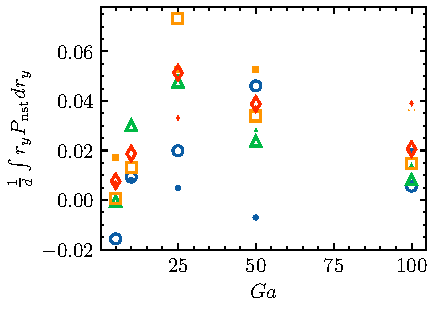
\includegraphics[height = 0.3\textwidth]{image/HOMOGENEOUS_NEW/PA/R.pdf}
    \caption{ First moment of the nearest particle pair distribution in the direction of gravity. 
    ($\pmb\bigcirc$) $\phi = 0.01$; ($\pmb\triangle$) $ \phi = 0.05$; ($\pmb\square$) $\phi = 0.1$ ($\pmb\lozenge$) $\phi = 0.2$.
    The hollow symbols correspond to $\lambda = 1$, the filled symbols to $\lambda = 10$.
    For $r<d$ we arbitrarily set $P_\text{r}^\text{th} = 1$ so that the distribution can be visualized.
    Black symbols represent the results of \citet{zhang2023evolution} for hard sphere suspension with $\phi = 0.016,0.056,0.134,0.262$  %$\phi = 0.0168,0.0565,0.1341,0.2622$ 
    corresponding to $\pmb\times,\pmb +, \pmb\star , \pmb\triangledown$, respectively.
    }
    \label{fig:ap:RY}
\end{figure}

\begin{figure}
  \centering
  \includegraphics[height = 0.3\textwidth]{image/HOMOGENEOUS_NEW/PA/rm.pdf}
  \caption{Dimensionless radial distance to the nearest neighbor for a random distribution.}
  \label{fig:ap:agee}
\end{figure}
% \section{Numerical validations}
% \label{ap:validation}
The \texttt{Basilisk} code has been validated numerous time in previous numerical studies. 
Especially, we can cite the recent studies of \citet{innocenti2020direct} and \citet{hidman2023assessing} which both performed DNS of rising suspension of bubbles. 
Nevertheless, in this work we investigate specific statistical distribution,
and we make use of a multi-VoF method to avoid droplets coalescence, therefore a meticulous validation of the DNS is in order. 
We start by presenting a brief comparison with the reference DNS \citet{esmaeeli1999direct}. 
Afterward we present a study focusing on the interfaces' kinematic, we compare our DNS with the experimental results of \citet{mohamed2003drop} in the objective to show that the Multi-VoF method indeed capture the physics of two colliding interfaces without solving the flows in the film. 
Once the mesh and the physics are validated, a study on the convergence of the statistics is presented. 

\subsection*{Ordered array of buoyant bubbles}

From our knowledge, no simulations nor experimental results have been carried out for rising buoyant viscous drop. 
Therefore, instead we reproduced the ordered array simulation of \citet{esmaeeli1999direct} with \texttt{Basilisk} to validate the mesh definition of our DNS.  
It consists in a 3-D buoyant ordered rising array of bubbles. 
In our notation the flow parameters of the simulation reads, 
\begin{align*}
    \lambda = 10,
    && \zeta = 10,
    && Bo = 1.8,
    && Ga = 28.37,
    && \phi = 0.125.
\end{align*}
\begin{figure}[h!]
    \centering
    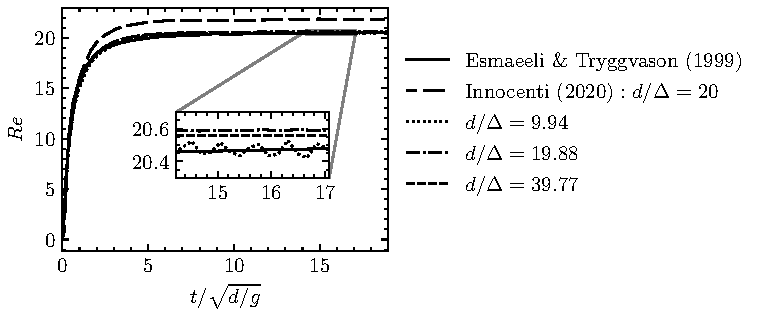
\includegraphics[height = 0.3\textwidth]{image/VALIDATION2.0/Loisy/Re.pdf}
    \caption{Time evolution of the Reynolds number based on the instentaneous volume averaged drift velocity, $Re(t) = \rho_fU d /\mu_f$, with $U(t) = |\textbf{u}_p - \textbf{u}_f|$ with $\phi = 0.1256$, $\zeta =\mu_r =10$ and $Ga = 29.9$.
    $\textbf{u}_p$ and $\textbf{u}_f$ are the particle and fluid phase volume averaged velocity at time $t$.}
    \label{fig:ordered_array}
\end{figure}
\ref{fig:ordered_array} display our numerical simulation against the original result of \citet{esmaeeli1999direct}.
We observe very good agreements between both studies for all mesh definition.
Additionally, we displayed the results of \citet{innocenti2020direct} for $d/\Delta = 20$ to point out a divergence with our results at the same mesh definition.  
Both our simulations and the one of \citet{innocenti2020direct} have been carried out with the  \texttt{Basilisk} code. 
The cause of this difference is in fact due to a different method of interpolation used for the viscosity coefficient $\mu$. 
We used an arithmetic mean, whereas \citet{innocenti2020direct} used a 
harmonic mean.
As a matter of fact in this regime the arithmetic mean, which will be used in this work, permit us to reach a faster convergence. 
Overall these results indicate that the criterion $d/\Delta = 30$ seems sufficient, which is consistent with the aforementioned studies.


\subsection*{Drop impact on a liquid-liquid interface}

In section, we investigate in more detail the physics behind the Multi-VoF method. 
We need to verify if we accurately capture the physics of the droplets interfaces despite the fact that we do not model accurately  the film between two droplets. 
Following \citet{balcazar2015multiple} we reproduced the experiment of drop impact on a liquid–liquid interface carried by \citet{mohamed2003drop} but with the \texttt{Basilisk} code. 
This experiment consist in letting a drop fall into a pool of the same fluid as the drop, all along the experiment the interfaces of the droplets and the pool are tracked. 
In our notation the dimensionless parameters of latter study reads, 
\begin{align*}
    Ga = 71.02 
    && Bo = 6.40
    && \lambda = 0.33
    && \zeta = 1.189
\end{align*}
Following \citet{mohamed2003drop} we defined the dimensionless time $t / t_i = t U_i(t) /d$ where $U_i(t)$ is droplet velocity at $t<0$ and where $t=0$ is the time of impact. 
Regarding the geometry of the problem we sketched in \ref{fig:schemeLong} a scheme of the initial position of the droplet in the computational domain.
Additionally, we displayed on \ref{fig:schemeLong} a snapshot of the numerical domain were we see the drop colliding the pool's interface.
Both, the drop and the pool does not merge since we use the Multi-VoF method, note that in the experiment the drop does not merge with the pool either.
This enables us to represent with DNS a physical situation where the interfaces do not coalesce, but where we use a grid definition of $d/\Delta = 30$ which is of course not sufficient to model the flow inside the film. 
\begin{figure}[h!]
    \centering
    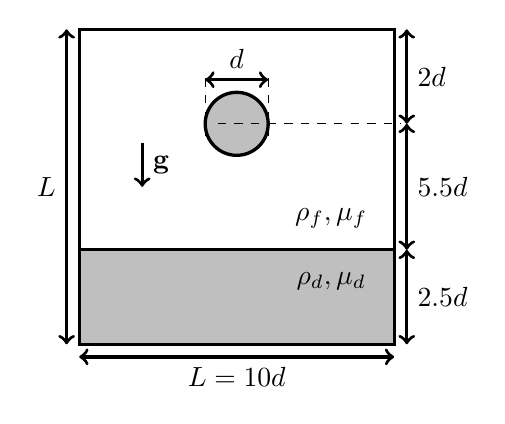
\begin{tikzpicture}[very thick,scale = 0.8]
        \draw (0,0) rectangle (5,5);
        \draw[fill=gray!50] (0,0) rectangle (5,1.5);
        \draw[fill=gray!50] (2.5,3.5) circle (0.5);
        \draw[<->](0,-0.2) --++ (5,0)node[midway,below]{$L  = 10 d$};
        \draw[<->](-0.2,0) --++ (0,5)node[midway,left]{$L$};
        \draw[<->](5.2,0) --++ (0,1.5)node[midway,right]{$2.5 d$};
        \draw[<->](5.2,1.5) --++ (0,2)node[midway,right]{$5.5 d$};
        \draw[<->](5.2,3.5) --++ (0,1.5)node[midway,right]{$ 2d$};
        \draw[dashed,thin](2.2,3.5) --++ (2.9,0);
        \draw[dashed,thin](2.2,3.5) --++ (2.9,0);
        \draw[->](1,3.2) --++ (0,-0.7)node[midway,right]{$\textbf{g}$};
        \draw[<->](2,4.2) --++ (1,0)node[midway,above]{$d$};
        \draw[thin,dashed](2,3.3) --++ (0,1);
        \draw[thin,dashed](3,3.3) --++ (0,1);
        \node (a) at (4,2){$\rho_f, \mu_f$};
        \node (a) at (4,1){$\rho_d, \mu_d$};
    \end{tikzpicture}
    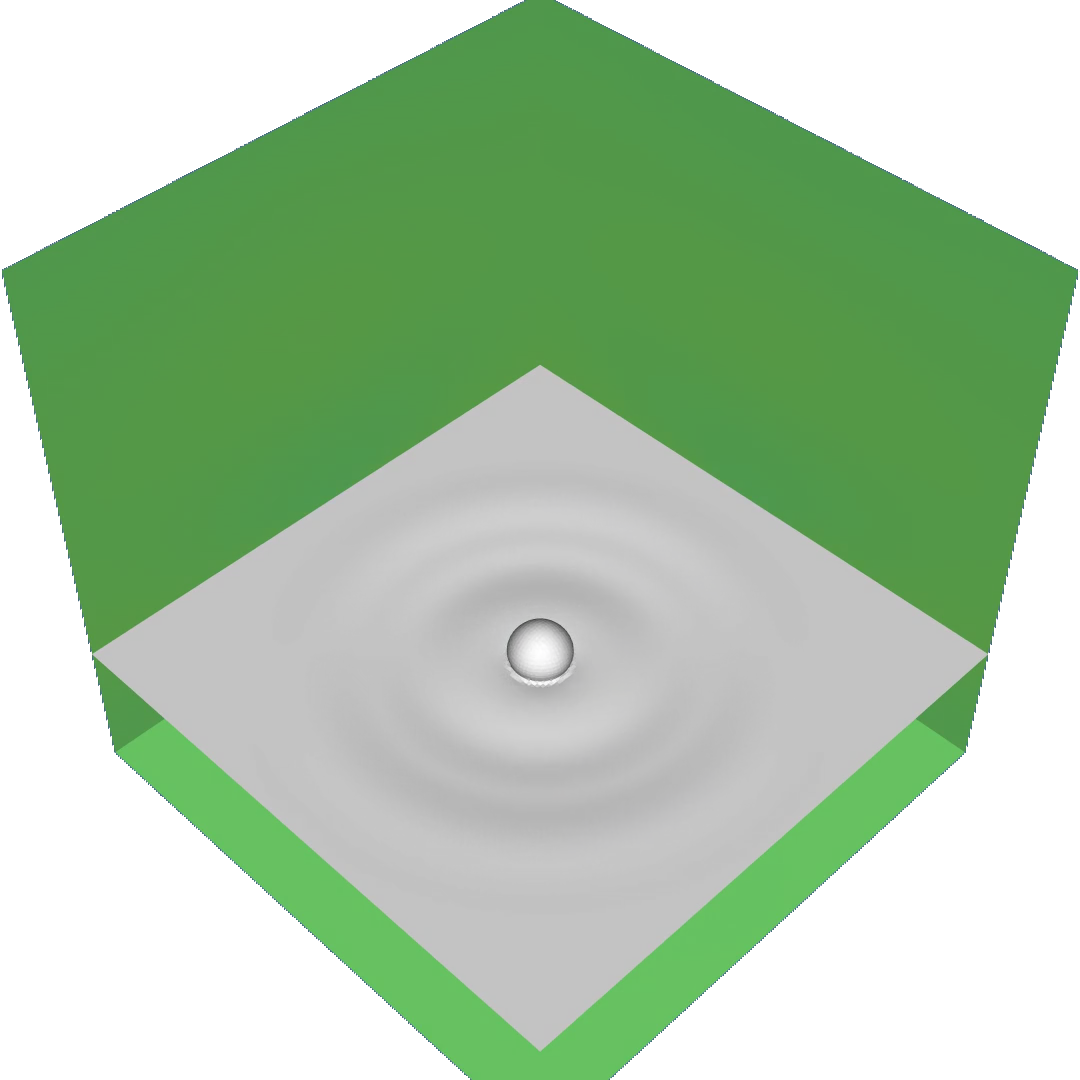
\includegraphics[height = 0.3\textwidth]{image/VALIDATION2.0/Longmire/IMG/image-079.png}
    \caption{(left) Scheme of the computational set up at the initial time. 
    (right) Snapshot of the computational domain after the collision time, with the interfaces represented in gray.
    The background color represent the velocity field magnitude, which is undisturbed, indicating a large enough domain. }
    \label{fig:schemeLong}
\end{figure}
\begin{figure}[h!]
    \centering
    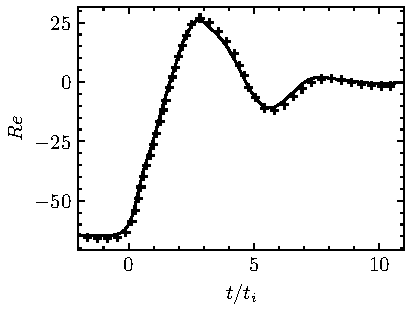
\includegraphics[height = 0.3\textwidth]{image/VALIDATION2.0/Longmire/Re.pdf}
    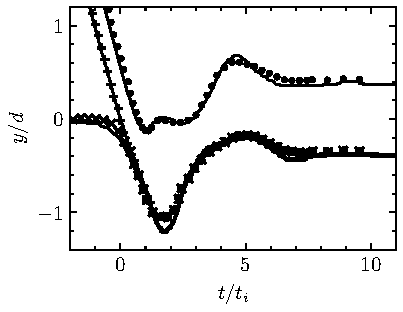
\includegraphics[height = 0.3\textwidth]{image/VALIDATION2.0/Longmire/Dist.pdf}
    \caption{(left) Time evolution of the Reynolds number based on the droplet velocity, $Re(t) = \rho_fU d /\mu_f$ in term of the dimensionless time, (+) numerical results of  \citet{balcazar2015multiple} (right)  position of the interfaces, ($\bullet$) top droplets surface, ($+$) bot droplet surface, (x) pool surface. (Symbols) experimental result of \citet{mohamed2003drop} (solid line) present numerical simulations with $d/\Delta = 30$. }
    \label{fig:resultslong}
\end{figure}
\ref{fig:resultslong} represent the comparison between our results against the experiment of \citet{mohamed2003drop} (right) and the numerical simulation of \citet{balcazar2015multiple} (left). 
The time dependent Reynolds number as well as the interfaces positions are shown to match exactly both, the numerical and experiential results of \citet{balcazar2015multiple} and \citet{mohamed2003drop}, respectively. 
From the very good agreement obtained with the numerical and experimental results we conclude that the kinematic is preserved during the contact time for a mesh definition of $d/\Delta = 30$. 

\subsection*{Mesh independence and statistical convergence for random array of drops}

Even through aforementioned studies carried validation of the \texttt{Basilisk} code for rising droplets or bubbles, almost all of them considered isolated droplets or bubbles as the only validation case. 
As far as the author's knowledge, to this date no published study presented a mesh independence study for random array of droplets nor bubbles of this scale. 
Nevertheless, as particles interaction and higher \textit{Galileo} numbers may be more challenging to model, it is primordial to investigate the mesh independence of the exact same DNS that are carried in this work. 
In this objective we performed DNS of random array of $N_b=125$ droplets, with the following parameters,
\begin{align*}
    \lambda = 10,
    && \zeta = 1.11,
    && Bo = 1,
    && Ga = 100,
    && \phi = 0.1,
    && N_b =125,
\end{align*}
and the mesh definition is, $d/\Delta = 7.37, 14.74, 29.9 58.97$. 
We expect that the most challenging DNS simulated in this work is for the case, $\lambda = 10$ and $Ga = 100$, since it is in this range of parameters that we induce the most vorticity, which ultimately require good mesh definition. 
Additionally, in opposition to the ordered array case, this case includes droplets interaction, which ultimately induce more numerical complexities to tackles. 
Based on this remark we can assume that if this case is mesh independent, then all cases from \ref{tab:simulations} must be since this is the most challenging scenario.   

Let's first verify the independence of the drift velocity on the mesh definition. 
\begin{figure}[h!]
    \centering
    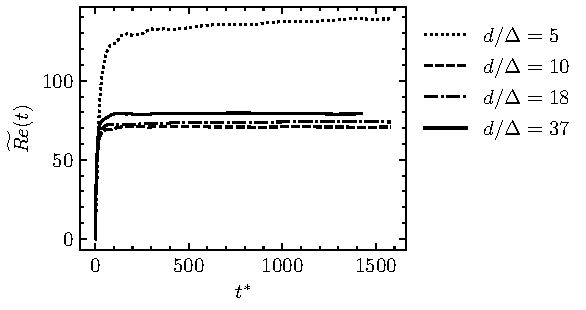
\includegraphics[height = 0.3\textwidth]{image/HOMOGENEOUS_NEW/VAL/Re.pdf}
    \caption{
        Time evolution of the Reynolds number based on the instantaneous volume averaged drift velocity, $Re(t) = \rho_fU d /\mu_f$, with $U(t) = |\textbf{u}_p - \textbf{u}_f|$ with $\phi = 0.1256$, $\zeta =\mu_r =10$ and $Ga = 29.9$ for different mesh definition.
        $\textbf{u}_p$ and $\textbf{u}_f$ are the particle and fluid phase volume averaged velocity at time $t$.
        In the legend we display the value of the mesh definition and of the ensemble averaged Reynolds number. 
    }
    \label{fig:Re}
\end{figure}
In \ref{fig:Re} we display the instantaneous volume averaged drift velocity in terms of time, for four mesh definition. 
The results are not as independent of the mesh definition as the order array validation presented above. 
Indeed, we observe a difference of the rising Reynolds number of about $5\%$ between the $d/\Delta = 29.49$ and $d/\Delta = 58.97$ cases which is notable.
We recall that this $5\%$ error will eventually be lower for all other cases. 
The good agreement between the case  $d/\Delta = 14.74$ and $d/\Delta = 29.49$ is partially fortuitous.

Now let's study the mesh influence on the statistics. 
It is clear from \ref{fig:apstat} (left) that both mesh definition produce nearly the same radial distribution, no notable difference is identified. 
In \ref{fig:ap_age} (middle) we can observe the age distribution for both mesh definition. 
It is clear that refining the mesh induce a difference in the age distribution. 
As, a matter of fact it has a small impact on the mean age, $\tau_p = 6.96$ for the lower definition, and $\tau_p = 6.14$ for the finest grid.
This makes a $10\%$ error, but as mentioned above this is probably the highest error that we could encounter among all cases. 
\begin{figure}
    \centering
    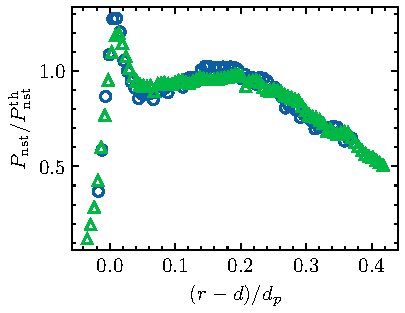
\includegraphics[height = 0.24\textwidth]{image/HOMOGENEOUS_NEW/VAL/Pr.pdf}
    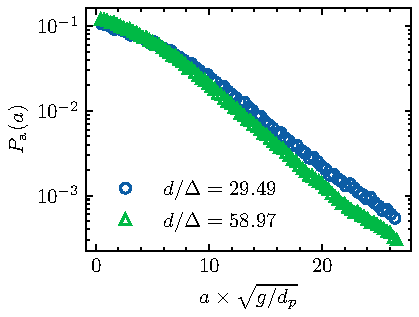
\includegraphics[height = 0.24\textwidth]{image/HOMOGENEOUS_NEW/VAL/Pa.pdf}
    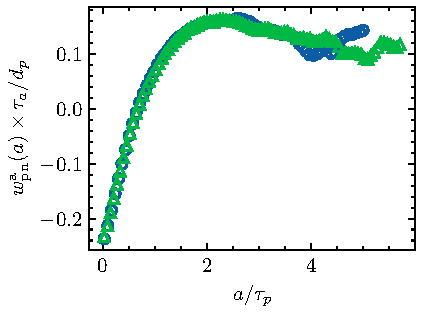
\includegraphics[height = 0.24\textwidth]{image/HOMOGENEOUS_NEW/VAL/w.pdf}
    \caption{
        Statistical averaged functions for two mesh definition. 
        (left) Radial normalized probability density function  $P_r(\textbf{x},|\textbf{r}|,t)/P_\text{th}$, in terms of the dimensionless radial position. 
        (middle) Probability density function of the age distribution $P_a(\textbf{x},t,a)$. 
        (right) Nearest averaged dimensionless approach velocity for both mesh definition, in terms of the dimensionless age. 
    }
    \label{fig:apstat}
\end{figure}
Even through an error is identified on the mean age of interaction we still notice that both nearest averaged dimensionless approach velocity on \ref{fig:apstat} (right) match perfectly. 
\begin{figure}[h!]
    \centering
    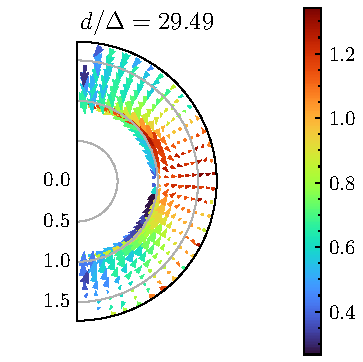
\includegraphics[height = 0.3\textwidth]{image/HOMOGENEOUS_NEW/VAL/U_rel_ndc_25.pdf}
    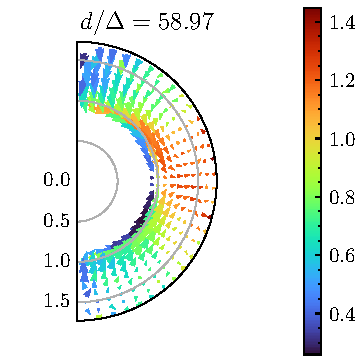
\includegraphics[height = 0.3\textwidth]{image/HOMOGENEOUS_NEW/VAL/U_rel_ndc_35.pdf}
    \caption{Quiver plots of the relative averaged velocity field $\textbf{w}^\text{r}(\textbf{x},\textbf{r},t)$ colored by the averaged dimensionless age $a^r(\textbf{x},\textbf{r},t)$, for $\phi = 0.05$ and $Ga = 100$. 
    (left) Low mesh definition.
    (right) High mesh definition. 
    }
    \label{fig:velap}
\end{figure}
Regarding, the 2D fields  $\textbf{w}^\text{r}(\textbf{x},\textbf{r},t)$ we can see that no notable difference can be identified, if it is not the slight difference in the value of the age scale. 


Overall, the one dimensional and two-dimensional conditioned statistics are almost independent of the mesh definition. 
By obtaining the same statistics with two independent DNS makes us confident on the fact that our numerical samples is large enough.
Indeed, if the samples were not sufficient we would have obtained two different distribution functions, thus we can be sure that the statistics have well converged. 
The slight difference in rising velocity and age distribution found for these Reynolds number must be acknowledged.
As mentioned at the beginning, this case is in fact very challenging as the volume fraction of droplets is consequent which induce numerous inertial interactions. 
Nevertheless, we can be sure that our final results is accurate at most with a $5\%$ error for this case, and probably less for the others cases. 
Overall, we have great confidence in the statistical and physical representativity of our DNS results. 


\bibliography{Bib/bib_bulles.bib}

\end{document}

